%
% komplexitaet.tex -- Kapitel ueber Komplexitaetstheorie
%
% (c) 2011 Prof Dr Andreas Mueller, Hochschule Rapperswil
%
\chapter{Komplexit"atstheorie\label{chapter-komplexitaet}}
\lhead{Komplexit"atstheorie}
\rhead{}
Im Kapitel \ref{chapter-entscheidbarkeit} wurde untersucht, ob ein
Problem "uberhaupt mit einer Turingmaschine l"osbar ist. Die
Effizienz der gewonnenen Algorithmen spielte keine Rolle.
In diesem Kapitel soll die Laufzeit eines Algorithmus genauer
untersucht werden. Dabei sind nur Unterscheidungen interessant,
die unabh"angig von den speziellen F"ahigkeiten der verwendeten
Maschine sind, nur so lassen sich allgemeing"ultige Aussagen
ableiten, die f"ur jede Art von Computer gelten. Die absolute Laufzeit
ist daher kein brauchbares Kriterium, sie h"angt zu stark
von individuell verschiedenen Parametern wie Taktrate, Wortbreite,
Instruktionssatz etc.~ab. 

Sobald ein geeignetes Kriterium gefunden werden kann, kann man
die Sprachen in ``leicht'' und ``schwierig'' zu entscheidende 
unterteilen. Dabei kristallisiert sich eine Klasse von
Problemen heraus, die von nichtdeterministischen Turingmaschinen
gerade noch gel"ost werden k"onnen, die aber f"ur grosse
Probleme ausserhalb der Reichweite von deterministischen Turingmaschinen
sind. Es scheint, dass diese Kluft nicht "uberbr"uckt werden kann.

F"ur die Praxis bedeutet dies, dass einige Probleme mit effizienten
Algorithmen gel"ost werden k"onnen, w"ahrend f"ur andere 
keine effizienten Algorithmen m"oglich sind. Der Praktiker wird daher
das Problem einschr"anken m"ussen, denn oft lassen sich solche
Probleme unter zus"atzlichen Bedingungen effizient l"osen.
Voraussetzung ist nat"urlich, dass er Probleme diesen beiden
Klassen zuordnen kann.

\section{Laufzeitkomplexit"at}
\rhead{Laufzeitkomplexit"at}
\index{Laufzeitkomplexit\"at}
\subsection{Inputl"ange}
\index{Inputl\"ange}
Wenn die absolute Laufzeit eines Algorithmus nicht als Mass f"ur
die Komplexit"at eines Problems dienen kann, dann vielleicht
wenigstens die Abh"angigkeit der Laufzeit von der Gr"osse des
Problems. Da wir unter Problemen immer ihre "Ubersetzung in ein
Sprachproblem verstehen, haben wir f"ur die Gr"osse des Problems
ein Mass: die L"ange des Wortes, welches das Problem beschreibt.

Als Beispiel betrachten wir das Problem
\index{PRIME@\textsl{PRIME}}
\[
\text{\textsl{PRIME}}=\{ n\;|\; \text{$n\in\mathbb N$ und $n$ ist prim}\}.
\]
Es ist entscheidbar, man kann zum Beispiel alle Teiler durchtesten,
das ist mit $n$ Tests m"oglich. Ein Entscheider ist also eine Turingmaschine,
der man die Zahl $n$ auf das Band schreibt, und die Turingmaschine
stellt dann fest, ob die Zahl eine Primzahl ist. Die Zahl $n$ muss
als String auf das Band geschrieben werden. Dazu ist eine Codierung
zu w"ahlen, "ublicherweise wird dies eine Zifferndarstellung in
irgendeiner Basis $b$ sein. Zur Darstellung der Zahl $n$ in Basis $b$
sind $l=\lfloor \log_bn\rfloor+1$ Zeichen notwendig.

Man k"onnte aber auch die un"are Darstellung verwenden, also so viele
$0$ auf das Band schreiben, wie die Zahl $n$ angibt. In dieser Codierung
ist also der Input wesentlich l"anger, n"amlich $l=n$.
F"ur die Beurteilung der
Komplexit"at kann also die Codierung des Inputs durchaus einen
merklichen Einfluss haben. Nehmen wir an, der Algorithmus hat
eine Laufzeit proportional zu $n$, dann w"achst die Laufzeit im
zweiten Fall proportional zur Inputl"ange $l$, im ersten Fall
aber w"achst die Laufzeit mit $b^l$. Man kann also Algorithmen
nur vergleichen, wenn man die gleiche Inputcodierung verwendet.

\subsection{Laufzeit}
\index{Laufzeit}
Sei jetzt also eine Turingmaschine $M$ gegeben, die ein Entscheider
ist. F"ur jedes Inputwort $w$ wird die Maschine eine gewisse Zeit
laufen und dann im Zustand $q_{\text{accept}}$ oder $q_{\text{reject}}$
anhalten. Die Anzahl der Rechenschritte, die die Maschine auf dem
Inputwort $w$ ben"otigt, bezeichnen wir mit $t(w)$.
Die maximale Laufzeit, die f"ur Inputw"orter der L"ange nicht
gr"osser als $n$ ben"otigt wird, bezeichnen wir mit $t(n)$,
\[
t(n)=\max \{ t(w)\;|\; |w|\le n\}.
\]
Der absolute Wert von $t(n)$ ist nicht interessant, da er sich
selbst unter trivialen Ver"anderungen der Turingmaschine ver"andern
kann. Das Verhalten von $t(n)$ f"ur grosse $n$ hingegen scheint
wesentlich robuster zu sein, es interessiert also nur noch, wie
sich verschiedene Funktionen zueinander verhalten, wenn man $n\to\infty$
streben l"asst. Falls wir die Turingmaschine angeben wollen, deren
Laufzeit bestimmt wird, schreiben wir sie als Index zu $t$: $t_M(n)$.

\begin{definition}
Sind $f$ und $g$ Funktionen $\mathbb N\to\mathbb R^+$, dann ist
$f(n)=O(g(n))$, falls es eine Konstante $c$ und ein $n_0\in\mathbb N$
gibt mit
\[
f(n)\le cg(n)\quad \forall n\in\mathbb N\text{ mit } n > n_0.
\]
Es ist $f(n)=O(g(n))$ wenn 
\begin{equation}
\lim_{n\to\infty}\frac{f(n)}{g(n)}=0.
\label{oquotientlimit}
\end{equation}
\end{definition}
\index{Laufzeit!polynomielle}
Man beachte, dass f"ur $f(n)=O(g(n))$ die Ungleichung $f(n)\le
cg(n)$ nicht f"ur alle $n$ gelten muss, insbesondere spielen kleine
Werte von $n$ keine Rolle, es interessiert uns nur das Verhalten
bei grossen Werten von $n$.
Und auch f"ur $f(n)=O(g(n))$ sind die kleinen Werte von $n$ nicht
von Bedeutung, die Funktionswerte f"ur kleine $n$ haben keinen
Einfluss auf den Grenzwert des Quotienten (\ref{oquotientlimit}).

Die Funktion $g$ muss offenbar nicht sonderlich genau bekannt
sein. Ist $g$ zum Beispiel ein Polynom, interessiert nur noch
die h"ochste Potenz. Es gilt ja zum Beispiel
$ n^r\le n^k $ f"ur jeden Exponenten $r<k$, und damit
$n^r=O(n^k)$. Ausserdem ist $an^r=O(n^k)$, und damit
f"ur $f(n)=a_0+a_1n+a_2n^2+\dots+a_{k-1}n^{k-1}+a_nn^k$ auch
$ f(n)=O(n^k) $. Somit gen"ugt es bei Polynomen f"ur $g$ die
h"ochste Potenz anzugeben.

\begin{beispiel}
F"ur das fr"uher genannte Beispiel \textsl{PRIME} wurde 2004 etwas
"uberraschend ein Algorithmus mit
polynomieller Laufzeit gefunden \cite{skript:aks}.
\end{beispiel}

\subsection{Varianten von Turingmaschinen}
Wieviel schneller arbeitet eine Turingmaschine mit mehreren B"andern 
gegen"uber einer Standardturingmaschine? Wieviel schneller ist eine
nichtdeterministische Turingmaschine gegen"uber einer deterministischen?

\begin{satz}
\index{Turing-Maschine!mit mehreren B\"andern}
Eine Turingmaschine mit mehreren B"andern und Laufzeit $t(n)$ kann
in Laufzeit $O(t(n)^2)$ auf einer Standardturingmaschine
simuliert werden.
\end{satz}

\begin{proof}[Beweis]
In Satz \ref{mehrbandturingmaschine} wurde beschrieben, wie man eine
Turingmaschine mit mehreren B"andern auf einer Turingmaschine mit
einem einzigen Band simulieren kann. Dabei ist f"ur jeden der
$t(n)$ Berechnungsschritt ein Durchgang durch das Band n"otig, bei
dem die Turingmaschine die Inhalte der markierten Felder zusammensammelt,
um dann die notwendigen "Anderungen zu bestimmen. Die "Anderungen
auf dem Band einzutragen erfordert dann nochmals einen Durchgang
durch das Band.

Wir nehmen an, dass $t(n)\ge n$, denn sonst k"onnte die
Turingmaschine nicht einmal ihren Input vollst"andig lesen.
Der tats"achlich benutzte Teil des Bandes kann dann nicht l"anger sein
als $t(n)$. Zusammen mit den $t(n)$ durchl"aufen erhalten wir,
dass die simulierte Turingmaschine die Laufzeit $O(t(n)^2)$ hat.
\end{proof}

Einen wesentlichen Unterschied der Laufzeit erwarten wir aber
bei nichtdeterministischen Turingmaschinen.
Die Berechnung in einer nichtdeterministischen Turingmaschine
kann ja auf ganz verschiedenen Wegen stattfinden, wovon
einer gefunden werden muss, der akzeptiert. Wenn eine simulierende
Turingmaschine alle Wege durchprobiert, spielt die Laufzeit auf
demjenigen Weg, der am l"angsten braucht, eine wesentliche Rolle.

\begin{definition}
\index{Laufzeit!einer nichtdeterministischen Turingmaschine}
Sei $N$ eine nicht deterministische Turingmaschine, die auch ein
Entscheider ist. Dann ist ihre Laufzeit $t(n)$ die maximale Anzahl
von Schritten, die jede m"ogliche Berechnung auf einem Input der
L"ange $\le n$ braucht.
\end{definition}

\begin{satz}
\label{exponentialtime}
Eine nichtdeterministische Turingmaschine mit Laufzeit $t(n)$
kann in Laufzeit $2^{O(t(n))}$
auf einer deterministischen Turingmaschine simuliert werden.
\end{satz}

\begin{proof}[Beweis]
In Satz \ref{nichtdeterministischeturingmaschine} wurde gezeigt,
wie man eine nichtdeterministische Turingmaschine auf einer
Mehrband-Maschine simulieren kann. Da wir im vorliegenden Fall
sogar einen Entscheider haben, k"onnen wir den Algorithmus noch
etwas vereinfachen. Wir verwenden Band~1 wieder f"ur den Input,
Band~2 als Arbeitsband f"ur die simulierte Turingmaschine und
Band~3 als Steuerband f"ur die nichtdeterministischen
Entscheidungen.

Wir m"ussen ausrechnen, wie sich die Simulation auf die 
Gesamtlaufzeit auswirkt. Jeder Berechnungspfad der simulierten
nichtdeterministischen Turingmaschine hat Laufzeit nicht
l"anger als $t(n)$. Die Erzeugung der n"achsten m"oglichen
Berechnungsgeschichte auf Band~3 kann in einem Durchgang
durch Band~3 erfolgen, braucht also Zeit $O(t(n))$.
Die Anzahl der Berechnungsgeschichten ist $|Q\times \Gamma|^{t(n)}$,
also von der Form $c^{t(n)}$. Im schlimmsten Fall ist die
Laufzeit dieses Algorithmus also
\[
c^{t(n)}(t(n) + O(t(n)))
=
2^{t(n) \log_2 c+ \log_2(O(t(n)))}
=
2^{O(t(n))}.
\]
\end{proof}
\subsection{Wie langsam ist exponentielle Laufzeit?}
\index{Laufzeit!exponentielle}
Satz \ref{exponentialtime} zeigt, dass zur Simulation eines
nichtdeterministischen Automaten eine exponentiell l"angere
Zeit n"otig ist, als die nichtdeterministische Maschine
ben"otigt h"atte. Aber wieviel langsamer ist das?
Zun"achst ist f"ur jeden Exponenten $k$
\[
\lim_{n\to\infty}\frac{2^{n}}{n^k}=\infty,
\]
$2^n$ w"achst also schneller als jedes Polynom. 
Setzen wir $t=n^r$, dann ist auch
\[
\lim_{n\to\infty}\frac{2^{n^r}}{n^k}
=
\lim_{t\to\infty}\frac{2^t}{t^{k/r}}
=
\infty,
\]
wie zu erwarten war, w"achst $2^{n^k}$ noch schneller.
Da nur schon f"ur das Lesen des Input $n$ Schritte notwendig sind,
spielt es gar keine Rolle, wie effizient der Algorithmus der
nichtdeterministischen Turingmaschine ist, es ist unm"oglich,
je polynomielle Laufzeit zu erreichen.

Aber wie gross ist denn nun exponentielle Laufzeit?
Nehmen wir an,
ein wir h"atten einen Algorithmus mit Laufzeit $n^k$. Vergr"ossert
man die Input-L"ange um $1$ Zeichen, "andert sich die Laufzeit um
\[
\frac{(n+1)^k}{n^k}
=
1+\frac{k}{n} +\dots,
\]
die relative Zunahme wird also immer kleiner. Bei einer Verdoppelung
der Inputl"ange wird die Laufzeit mit dem Faktor $2^k$ multipliziert.
Ganz anders bei exponentieller Laufzeit.
Erh"oht man die Inputl"ange um $1$, wird die Laufzeit mit einem
konstanten Faktor multipliziert. Und die Verdoppelung von $n$
quadriert die Laufzeit.
Ausgehend von einer angenommenen
Zeit pro Schritt von einer Nanosekunde, ergeben sich
f"ur die Laufzeit eines Algorithmus
mit polynomieller Laufzeit, genauer mit $n^5$ und exponentieller Laufzeit,
genauer mit $2^n$ die Werte in Tabelle~\ref{laufzeittabelle}.
\begin{table}[H]
\begin{center}
\begin{tabular}{|l|rr|}
\hline
$n$&$n^5$&$2^n$\\
\hline
  1&             1ns&             2ns\\
  2&            32ns&             4ns\\
  4&       1.0$\mu$s&            16ns\\
  8&      32.7$\mu$s&           256ns\\
 16&           1.0ms&      65.5$\mu$s\\
 32&          33.5ms&           4.3ms\\
 64&            1.0s&       584 Jahre\\
128&           34.4s& $10^{21}$ Jahre\\
\hline
\end{tabular}
\end{center}
\caption{Polynomielle und exponentielle Laufzeit\label{laufzeittabelle}}
\end{table}
Die Zeit von $10^{21}$ Jahren entspricht dem 78 Milliardenfachen des
Alters des Universums. Grosse Probleme mit exponentieller Laufzeit
sind also schlicht unl"osbar, w"ahrend selbst relativ grosse
polynomielle Laufzeiten durchaus im Bereich des erreichbaren sind.
Der Unterschied zwischen polynomieller und exponentieller Laufzeit
ist also f"ur grosse Inputl"ange der Unterschied zwischen l"osbaren und
unl"osbaren Problemen.

\section{Klassen P und NP}
\index{Klasse P}
\rhead{Klassen P und NP}
\subsection{Klasse P}
Bei der Simulation einer Turingmaschine mit mehreren B"andern
auf einer Standardmaschine wird die Laufzeit im schlimmsten
Fall quadriert. Die Funktion $t_M(n)$ ist also keine Invariante
in der Menge der entscheidbaren Sprachen. F"ur das gleiche Problem kann
je nach eingesetztem Maschinentyp ein v"ollig anderes Laufzeitverhalten
beobachtet werden. 

Erhalten bleibt aber die Eigenschaft der Funktion $t_M(n)$, 
polynomiell zu sein. Simuliert man eine Turingmaschine $M_1$ mit
mehreren B"andern auf einer Standardturingmaschine $M_2$,
dann ist $t_{M_2}=O(t_{M_1}(n)^2)$.
Wenn also $t_{M_1}(n)=O(n^k)$ ist, dann ist $t_{M_2}(n)=O(n^{2k}).$
Beide Maschinen haben eine Laufzeit, die durch ein Polynom beschr"ankt
sind.

\begin{definition}
\index{Klasse P}
Die Klasse $P$ besteht aus den Sprachen, die mit einem Entscheider
mit polynomieller Laufzeit entschieden werden k"onnen.
\end{definition}

\subsection{Beispiele von Sprachen in P}
\index{Sprachen!kontextfreie}
\begin{satz}
Kontextfreie Sprachen sind in P.
\end{satz}

Der Satz besagt, dass es zu jeder kontextfreie Sprache eine
Turingmaschine gibt, die die Zugeh"origkeit eines Wortes zur
Sprache in einer Zeit entscheiden kann, die polynomiell ist in
der L"ange des Wortes.

\begin{proof}[Beweis]
Der CYK-Algorithmus aus Satz \ref{cyk-algorithm}
kann in Zeit $O(n^3)$ durchgef"uhrt werden.
\end{proof}

Sei $G$ ein gerichteter Graph und $s$ und $t$ zwei Vertizes
des Graphen. Das Pfad-Problem fragt, ob es einen von $s$ nach $t$
f"uhrend Pfad in dem Graphen gibt. "Ubersetzt in ein Spracheproblem
liefert es uns den folgenden Satz.

\begin{satz}
\index{PATH@\textsl{PATH}}
Die Sprache
\[
\text{\textsl{PATH}}
=\{
\langle G,s,t\rangle
\;|\;\text{$G$ ist ein gerichteter Graph mit einem Pfad von $s$ nach $t$}
\}
\]
ist in P.
\end{satz}

\begin{proof}[Beweis]
\index{Markierungsalgorithmus}
Ein Markierungsalgorithmus, der beginnend bei $s$ alle erreichbaren
Vertizes markiert, solange sich noch neue Vertizes markieren lassen,
hat polynomielle Laufzeit.
\end{proof}

\begin{satz}
\index{RELPRIM@\textsl{RELPRIME}}
Die Sprache
\[
\text{\textsl{RELPRIME}}
=\{
\langle a,b\rangle \;|\;
\text{$a, b\in \mathbb N$ und $a$ und $b$ sind teilerfremd}
\}
\]
ist in P.
\end{satz}

\begin{proof}[Beweis]
\index{Algorithmus!euklidischer}
Teilerfremdheit kann mit dem euklidischen Algorithmus entscheiden werden.
Dieser funktioniert wie folgt:
\begin{compactenum}
\item Wiederhole Schritte 2 und 3 bis $y=0$:
\item Weise $x$ den Wert $x\mod y$ zu
\item Vertausche $x$ und $y$
\item Gebe Resultat $x$ zur"uck.
\end{compactenum}
Bei diesem Algorithmus wird $x$ in jedem Schritt mindestens halbiert,
die Laufzeit ist also proportional zur gr"osseren der
beiden Zahlen $\log_2 a$ und $\log_2 b$, also ist die Laufzeit
polynomiell in der Inputl"ange $\log_2 a+\log_2 b$.
\end{proof}

\subsection{Verifizierer}
Sprachen, die von einer nichtdeterministischen Turingmaschine
in polynomieller Zeit entschieden werden, brauchen bei der
Simulation auf einer deterministischen Turingmaschine im
schlimmsten Fall exponentiell l"anger. Es ist also im
allgemeinen fast unm"oglich, ein solches Problem zu l"osen.

Gibt man allerdings die L"osung vor, zum Beispiel indem man
die richtigen nichtdeterministischen Entscheidungen vorgibt,
kann man die Probleml"osung in polynomieller Zeit nachvollziehen.
Genau diese Idee formalisiert das Konzept des Verifizierers.

\begin{definition}
\index{Verifizierer}
Ein Verifizierer f"ur die Sprache $A$ ist eine Turingmaschine
$V$ mit
\[
A=\{
w\;|\;\text{$\exists c\in C^*$ so dass $V$ $\langle w,c\rangle$ akzeptiert}
\},
\]
wobei $C$ eine endliche Menge ist.
Ein Verifizierer heisst polynomiell, wenn seine Laufzeit polynomiell
ist in der L"ange des Wortes $w$.
\end{definition}

Man beachte, dass die L"ange von $c$ auf die Laufzeit keinen
Einfluss haben darf. Der Verifizierer muss n"amlich gar nicht
den ganzen String $c$ anschauen, er muss davon nur soviel
nehmen, wie er f"ur die Verifikation braucht. Aber nat"urlich
muss er den ganzen String $w$ lesen, von dessen L"ange muss
die Laufzeit abh"angen.

Ein Verifizierer ist erst n"utzlich, wenn man auch $c\in C^*$
hat. Im Falle des Akzeptanzproblems durch eine nichtdeterministische
Turingmaschine (siehe Einf"uhrungsbeispiel) kann die Folge der
nichtdeterministischen Entscheidungen in der Berechnung diese
Funktion "ubernehmen. Daraus schliessen wir

\begin{satz} Eine Sprache wird genau dann von einer
nichtdeterministischen Turingmaschine in polynomieller Zeit entschieden,
wenn sie einen polynomiellen Verifizierer hat.
\end{satz}

\begin{proof}[Beweis]
Bereits gezeigt haben wir, dass eine nichtdeterministisch in
polynomieller Zeit entscheidbare Sprache einen polynomiellen Verifizierer hat.
Es ist also
nur noch zu kl"aren, dass auch das Umgekehrte gilt, dass also eine
Sprache mit einem polynomiellen Verifizierer nichtdeterministisch
in polynomieller Zeit entschieden werden kann.

Dazu verwenden wir den folgenden Entscheidungsalgorithmus:
\begin{compactenum}
\item Erzeuge nicht deterministisch $c\in C^*$.
\item Teste, ob $V$ $\langle w,c\rangle$ akzeptiert.
\item falls $V$ akzeptiert: $q_{\text{accept}}$, falls nicht:
$q_{\text{reject}}$
\end{compactenum}
Die Laufzeit dieses Algorithmus wird bestimmt von der Laufzeit von $V$,
ist also polynomiell in der L"ange von $w$.
\end{proof}

\begin{beispiel}[Faktorisierung]
Die Faktorisierung eines Produktes von zwei grossen Primzahlen
gilt allgemein als schwierig. Die Sicherheit des RSA-Algorithmus,
der in zahlreichen im Internet verbreiteten kryptographischen
Protokollen verwendet wird, basiert wesentlich auf der Tatsache, dass
es sehr einfach ist, ein Produkt von zwei grossen Primzahlen zu
bilden, aber sehr viel schwieriger, aus dem Produkt die beiden
Faktoren wieder zu ermitteln.

Es geht also um die Sprache
\[
L
=
\{
n\;|\,\text{$n=pq$, wobei $p$ und $q$ Primzahlen sind}.
\}
\]
Erfahrungsgem"ass ist es praktisch unm"oglich, die Faktoren
einer Zahl in $n$ zu bestimmen, und damit zu entscheiden, ob
$n\in L$ ist. Kennt man jedoch einen der beiden Faktoren,
zum Beispiel $p$, dann kann man mit dem Divisionsalgorithmus
nachpr"ufen, ob die Division ``aufgeht'', was in einer Anzahl
von Schritten m"oglich ist, die proportional zur L"ange von 
$n$, also zu $\log_b n$ ist. Der Test auf Rest 0 bei Teilung
durch $p$ ist also ein polynomieller Verifizierer mit $c=p$.
\end{beispiel}

\subsection{Klasse NP}
Keine Variante der Turingmaschine macht aus einem Problem,
welches sich in einer Laufzeit $2^{O(n^k)}$ entscheiden
l"asst, ein Problem in $P$. Es ist daher zu vermuten,
dass die Sprachen, die nichtdeterministisch in polynomieller
Zeit entschieden werden k"onnen, eine wesentlich gr"ossere
Klasse bilden als $P$.

\begin{definition}
\index{Klasse NP}
Die Klasse der von einer nichtdeterministischen Turingmaschine
in polynomieller Zeit entscheidbaren Sprachen heisst NP.
\end{definition}

\begin{figure}[H]
\begin{center}
\includegraphics{images/lang-5}
\end{center}
\caption{Jede Sprache in P ist auch in NP\label{psubsetnp}}
\end{figure}%

Insbesondere enth"alt NP alle Sprachen mit einem polynomiellen
Verifizierer. Es ist auch klar, dass $\text{P}\subset\text{NP}$,
siehe Abbildung \ref{psubsetnp}.
Ein offenes Problem ist jedoch, ob $\text{P}\ne \text{NP}$.
Die Bedeutung dieser Frage wird sp"ater klar werden.

\subsection{Satisfiability: \textsl{SAT}}
\index{SAT}
\index{Satisfiability}
Die Sprache 
\[
\text{\textsl{SAT}}=\{\varphi\;|\;\text{$\varphi$ ist eine erf"ullbare logische Formel}\}
\]
ist entscheidbar. F"ur eine logische Formel $\varphi(x_1,\dots,x_n)$
testet man einfach alle m"oglichen Belegungen der Variablen $x_1,\dots,x_n$
mit Wahrheitswerten.
Daf"ur sind $2^n$ Verifikationen notwendig, dies ist also
bestimmt kein Algorithmus in P.

\textsl{SAT} ist aber in NP,
denn wir k"onnen einen polynomiellen Verifizierer angeben.
Der Verifizierer verlangt als L"osungszertifikate $c$ eine
Belegung der Variablen mit Wahrheitswerten $c=(x_1,\dots,x_n)$,
und "uberpr"uft, ob durch einsetzen der Werte $x_1,\dots,x_n$
die Formel $\varphi(x_1,\dots,x_n)$ wahr wird.

Eine Variante von \textsl{SAT} ist \textsl{3SAT}.
Im Gegensatz zu \textsl{SAT} enth"alt \textsl{3SAT}
nur Formeln in konjunktiver Normalform, und jede Klausel
enth"alt genau drei Terme (3cnf-Formel).
Eine typische Formel in \textsl{3SAT} ist 
\[
\varphi=(x_1\vee x_2\vee x_3)\wedge (\bar x_1\vee x_3\vee \bar x_4)\wedge
	(x_1\vee x_3\vee x_5).
\]
Die Sprache \textsl{3SAT} ist
\[
\text{\textsl{3SAT}} =\{\varphi\;|\; \text{$\varphi$ ist eine erf"ullbare 3cnf-Formel}\}.
\]
Wie \textsl{SAT} ist \textsl{3SAT} in NP.

\subsection{Existenz von Cliquen: \texorpdfstring{$k$}{k}-\textsl{CLIQUE}}
\begin{figure}[H]
\begin{center}
%\includegraphics[width=0.6\hsize]{images/comp-1}
\includegraphics[width=0.35\hsize]{images/comp-1}
\end{center}
\caption{Graph mit sechs Knoten, keiner 4-Clique, aber
vier 3-Cliquen\label{6graph}}
\end{figure}%
\begin{figure}[H]
\begin{center}
\begin{tabular}{cccc}
\includegraphics[width=0.35\hsize]{images/comp-2}&%
\includegraphics[width=0.35\hsize]{images/comp-3}\\
\includegraphics[width=0.35\hsize]{images/comp-4}&%
\includegraphics[width=0.35\hsize]{images/comp-5}
\end{tabular}
\end{center}
\caption{3-Cliquen des Graphen von Abbildung~\ref{6graph}}
\end{figure}%
\index{Clique}
\index{Clique@$k$-Clique}
\index{Cliquen-Problem}
\index{CLIQUE@\textsl{CLIQUE}}
Eine $k$-Clique in einem Graph $G$ ist eine Menge von $k$
Ecken des Graphen so, dass in $G$ jede Ecke der Teilmenge mit
jeder anderen Ecke verbunden ist. Im umgangssprachlichen Gebrauch
ist eine Clique eine Gruppe von Leuten, in der jeder jeden kennt.

Das Cliquen-Problem
\[
\text{$k$-\textsl{CLIQUE}} = \{ \langle G\rangle\;|\;
\text{$G$ ist eine Graph mit einer $k$-Clique}\}
\]
ist entscheidbar. Man probiert alle m"oglichen $k$-elementigen
Teilmengen der Ecken des Graphen durch, ob sie eine Clique
bilden. Da Zahl der Teilmengen ist $\binom{n}{k}$, wenn $n$
die Zahl der Ecken ist, und $\binom{n}{k}$ von der Gr"ossenordnung
$O(n^k)$ ist, ist dieser Algorithmus nicht in P.

Das Cliquen-Problem ist aber in NP. Dazu muss wieder ein
Verfizierer angegeben werden. Als L"osungszertifikat verlangt
der Verifizierer die Menge $c=\{v_1,\dots,v_k\}$ der
Vertizes, die angeblich eine $k$-Clique bilden. Dann testet
er jedes Paar von Vertices in $c$ daraufhin, ob sie in $G$
verbunden sind. Dies sind weniger als $k^2$ Tests die nicht
weniger Aufwand als die Gr"osse des Graphen brauchen, die
Komplexit"at dieses Algorithmus ist also $O(n)$, das
Cliquen-Problem ist in NP.

\subsection{F"arbeproblem: \texorpdfstring{$k$}{k}-\textsl{VERTEX-COLORING}}
\index{F\"arbeproblem}
\begin{figure}[H]
\begin{center}
\begin{tabular}{ccc}
\includegraphics{images/comp-6}&
\qquad&\qquad
\includegraphics{images/comp-7}
\end{tabular}
\end{center}
\caption{Zum F"arbeproblem: der Graph links kann mit drei Farben
eingef"arbt werden, der Graph rechts braucht vier verschiedene Farben
\label{vertex-coloring-examples}}
\end{figure}%
\index{VERTEX-COLORING@\textsl{VERTEX-COLORING}}
Man sagt, die Vertizes eines Graphen $G$ k"onnen mit $k$ Farben
eingef"arbt werden, wenn sich f"ur jeden Vertex eine der $k$ Farben
w"ahlen l"asst, so dass nie zwei durch eine Kante verbundene Vertizes
die gleiche Farbe bekommen.

Das F"arbe-Problem 
\[
\text{$k$-\textsl{VERTEX-COLORING}}
=
\{
\langle G\rangle\;|\;
\text{$G$ ist ein mit $k$ Farben einf"arbbarer Graph}\}
\}
\]
ist entscheidbar. Man kann alle $k^n$ m"oglichen F"arbungen
($n$ die Anzahl der Vertizes) durchtesten, ob sie die Bedingung
erf"ullen, dass verbundene Vertizes nicht die gleiche Farbe haben
d"urfen.

$k$-\textsl{VERTEX-COLORING} ist in NP, denn ein polynomieller Verifizierer
wird als L"osungszertifikat die Farbzuordnung $c=(c_1,\dots,c_n)$ der
Ecken $1,\dots,n$ des Graphen verlangen, und kann damit in polynomieller
Zeit pr"ufen, ob die Bedingung verschiedener Farbe an den Enden
jeder Kante erf"ullt ist.

\section{Reduktion}
\rhead{Reduktion}
Die Beispiele des vorangegangenen Abschnittes haben gezeigt,
dass der Nachweis, dass eine Sprache in P ist, mit grossem
Aufwand verbunden sein kann, weil ein geeigneter Algorithmus
gefunden werden muss. Ein "ahnliches Problem konnte in der
Entscheidungstheorie durch die Verwendung einer Reduktionsabbildung
$f\colon A\le B$
gel"ost werden. Eine solche musste berechenbar sein, und erlaubte
die Entscheidung, ob ein Wort in $A$ ist, in die Sprache
$B$ zu transportieren, und dort zu entscheiden.

Im Zusammenhang der Komplexit"at m"ochte man das ebenfalls
tun, doch muss die Reduktionsabbildung jetzt auch noch 
polynomielles Laufzeitverhalten haben, damit sie n"utzlich
bleibt.

\begin{definition}
\index{Reduktion}
Eine berechenbare Abbildung $f\colon \Sigma^*\to\Sigma^*$
mit den Eigenschaften
\begin{compactenum}
\item $w\in A\quad\Leftrightarrow\quad f(w)\in B$
\item Es gibt eine Turingmaschine mit polynomieller Laufzeit, die
$f(w)$ berechnet.
\end{compactenum}
heisst eine polynomielle Reduktion $A\le_P B$.
\end{definition}

\begin{satz}
\label{polynomiellreduction}
Ist $A\le_P B$ und $B$ in P, dann ist auch $A$ in P.
\end{satz}

\begin{proof}[Beweis]
Da $B\in\text{P}$ gibt es eine Turingmaschine $M$ mit polynomieller Laufzeit,
die $w\in B$ entscheiden kann. Der folgende Algorithmus entscheidet
jetzt auch $w\in A$:
\begin{compactenum}
\item Berechnen $f(w)$
\item Wende $M$ auf $f(w)$ an.
\end{compactenum}
Wir m"ussen uns nur noch versichern, dass dieser Algorithmus 
polynomielle Laufzeit hat. Die Laufzeit der Turingmaschine ist
$t_M(|f(w)|)$. Aber $|f(w)|$ kann nicht l"anger als die Laufzeit 
der Berechnung von $f(w)$ sein, man kann ja in jedem Schritt h"ochstens
ein Zeichen schreiben. Schreiben wir $t_f(n)$ f"ur die Laufzeit
der Berechnung von $f$, ist die Gesamtlaufzeit des Algorithmus
$t_M(t_f(|w|))$. Sowohl $t_M$ als auch $t_f$ sind Polynome, 
also ist auch die Zusammensetzung ein Polynom, der Algorithmus
hat somit polynomielle Laufzeit.
\end{proof}

\begin{satz}
Ist $A\le_P B$ und hat $B$ einen polynomiellen Verifizierer, dann
hat auch $A$ einen polynomiellen Verifizierer. Falls $A\le_P B$ und 
$B\in\text{NP}$, dann ist auch $A\in\text{NP}$.
\end{satz}

\begin{proof}[Beweis]
Aus einem polynomiellen Verifizierer $V$ f"ur $B$ kann man durch
Zusammensetzen mit der Reduktionsabbildung $f\colon A\le_P B$
einen polynomiellen Verifizierer f"ur $A$ konstruieren.
\end{proof}

Die letzten zwei S"atze zeigen, dass sich Sprachen in $P$ und $NP$
mit Hilfe der polynomiellen in ``leichte'' und ``schwierige'',
in ``schnell'' bzw.~``langsam'' zu l"osende unterteilen lassen
(Abbildung \ref{pnporder}).
\begin{figure}[H]
\begin{center}
\includegraphics{images/lang-6}
\end{center}
\caption{Sprachen werden durch die polynomielle Reduktion $\le_P$
nach ``Schwierigkeit'' geordnet.\label{pnporder}}
\end{figure}%

\begin{beispiel}[\bf Stundenplan und das F"arbeproblem]
\index{Stundenplanproblem}
Das Studenplanproblem $S$ besteht darin
einen Stundenplan so zu erstellen, dass die Studenten alle
Vorlesungen besuchen k"onnen, f"ur die sie sich angemeldet haben.
Die Lektionen m"ussen dabei auf Zeitfenster verteilt werden,
so dass es keine Kollisionen gibt.

Um dieses Problem zu l"osen, muss man es auf ein bekanntes
Problem reduzieren. In diesem Fall bietet sich das Eckenf"arbeproblem
\textsl{VERTEX-COLORING}
f"ur Graphen an. Es wird verlangt, die Ecken eines Graphen mit 
verschiedenen Farben so einzuf"arben, dass keine zwei benachbarten
Ecken die gleiche Farbe haben.

Den verf"ugbaren Zeitfenstern f"ur Lektionen m"ussen die F"acher zugeordnet werden
so, dass kein Student zwei F"acher im gleich Zeitfenster
besuchen will.
Die Lektionen bilden als Ecken eines Graphen, zwischen zwei
Ecken gibt es eine Kante, wenn ein Student sich f"ur beide 
Lektionen angemeldet hat. Den Lektionen m"ussen jetzt Zeitfenster
zugeordnet werden, so dass es keine Kollisionen gibt, die
Zeitfenster sind also die Farben, mit denen die Ecken  des
Graphen eingef"arbt werden sollen. Die Einf"arbung ist genau
dann m"oglich, wenn es eine L"osung f"ur das Stundenplanproblem gibt.
Damit haben wir eine Abbildung konstruiert
\[
\begin{tabular}{>{$}r<{$}>{$}c<{$}>{$}l<{$}}
S&\to&\text{$k$-\textsl{VERTEX-COLORING}}\\
\text{Fach}&\mapsto&\text{Vertex}\\
\text{Zeitfenster}&\mapsto&\text{Farbe}\\
\text{Anzahl Zeitfenster}&\mapsto&k\\
\text{Student/Anmeldung}&\mapsto&\text{Kante}
\end{tabular}
\]
Diese Abbildung ist offenbar eine polynomielle Reduktion
\[
S\le_P \text{$k$-\textsl{VERTEX-COLORING}}.
\]
Die Reduktion kann aber auch in umgekehrter Richtung erfolgen,
es gibt also auch eine Reduktion
\[
\text{$k$-\textsl{VERTEX-COLORING}}\le_P S.
\]
\end{beispiel}

\begin{beispiel}[\bf\textsl{3SAT} und \textsl{CLIQUE}]
Eine $k$-Clique in einem Graphen ist ein vollst"andiger
Untergraph mit $k$ Ecken in einem gegebenen Graphen. Im Cliquen-Problem m"ussen
in einem gegebenen Graphen $k$ Ecken gefunden werden, so dass
jede m"ogliche Verbindung zwischen den Ecken auch im Graphen $G$ 
besteht. Als Sprache formuliert, ist es
\[
\text{\textsl{CLIQUE}}
=\{
\langle G,k\rangle\;|\;\text{$G$ ist ein Graph mit einer $k$-Clique}
\}
\]
Wir konstruieren jetzt eine Reduktion 
\[
\text{\textsl{3SAT}}\le_P
\text{\textsl{CLIQUE}}
\]
Man muss also aus jeder Formel in konjunktiver Normalform mit
drei Klauseln einen Graphen konstruieren, der genau dann eine
$k$-Clique besitzt, wenn die Formel erf"ullbar ist. Ausserdem
muss die Konstruktion in polynomieller Zeit durchf"uhrbar sein.

Sei also die Formel von der Form
\[
\varphi
=
\varphi_1\wedge\varphi_2\wedge\dots\wedge\varphi_k,
\]
wobei jede Teilformel $\varphi_i$ nur eine Disjunktion (Oder-Verkn"upfung)
von Variablen oder negierten Variablen ist. Damit $\varphi$
erf"ullbar ist, muss es eine Zuordnung von Wahrheitswerten zu
den Variable geben, so dass jede der Teilformeln $\varphi_i$ wahr
wird. In jeder Teilformel gibt es also eine Variable oder 
negierte Variable, die wahr ist. Es w"urde also gen"ugen,
die Terme in den $\varphi_i$ zu finden, die alle gleichzeitig
wahr sein k"onnen.

Wir konstruieren jetzt den Graphen wie folgt. Die Ecken des Graphen
sind die Variablen der Teilformeln $\varphi_i$. Eine Kante wird
eingezeichnet f"ur jedes Paar von Variablen in verschiedenen
Teilformeln, die gleichzeitig wahr sein k"onnen. Die Formel $\varphi$
ist genau dann erf"ullbar, wenn der Graph eine $k$-Clique enth"alt.

\begin{figure}[H]
\[
\entrymodifiers={++[o][F]}
\xymatrix{
*+\txt{}
	&{\bar x_1}
		\ar@{-}[dl] \ar@{-}[ddl] \ar@{-}[dddl]
		\ar@{-}[dddd] \ar@{-}[ddddr] 
		%\ar@{-}[drrr]
		\ar@{-}[ddrrr] \ar@{-}[dddrrr]
		&{\bar x_2}
			\ar@{-}[dddll]
			\ar@{-}[ddddl] \ar@{-}[dddd] \ar@{-}[ddddr]
			\ar@{-}[drr] \ar@{-}[dddrr]
			\ar@{-}[dll] \ar@{-}[ddll]
			&{x_2}
				\ar@{-}[dddlll] \ar@{-}[dddlll]
				\ar@{-}[dddd]
				\ar@{-}[dr] \ar@{-}[ddr]
\\
{\bar x_2}
	\ar@{-}[rrrr] \ar@{-}[rrrrdd]
	\ar@{-}[dddr] \ar@{-}[dddrr] \ar@{-}[dddrrr]
	&*+\txt{}
		&*+\txt{}
			&*+\txt{}
				&{\bar x_1}
					\ar@{-}[dllll] \ar@{-}[ddllll]
					\ar@{-}[dddlll] \ar@{-}[dddll]
\\
{\bar x_2}
	\ar@{-}[rrrrd]
	\ar@{-}[ddr] \ar@{-}[ddrr] \ar@{-}[ddrrr]
	&*+\txt{}
		&*+\txt{}
			&*+\txt{}
				&{x_2}
					\ar@{-}[dllll]
					\ar@{-}[ddl]
\\
{\bar x_1}
	\ar@{-}[rrrr]
	\ar@{-}[dr] \ar@{-}[drr]
	&*+\txt{}
		&*+\txt{}
			&*+\txt{}
				&{\bar x_2}
					\ar@{-}[dlll] \ar@{-}[dll] \ar@{-}[dl]
\\
*+\txt{}
	&{\bar x_2}
		&{\bar x_2}
			&{x_1}
}
\]
\caption{Graph zur Formel $\varphi$\label{phiformel}}
\end{figure}%
Als Beispiel f"ur die Konstruktion des Graphen nehmen wir die Formel
\[
\varphi
=
(\bar x_1\vee \bar x_2\vee x_2)
\wedge
(\bar x_1\vee x_2\vee \bar x_2)
\wedge
(x_1\vee \bar x_2\vee \bar x_2)
\wedge
(\bar x_1\vee \bar x_2\vee \bar x_2)
\]
Der nach obigen Regeln konstruierte Graph ist in Abbildung~\ref{phiformel}
dargestellt.
Nat"urlich enth"alt dieser Graph gen"ugend Kanten, so dass es relativ
leicht ist, eine $4$-Clique zu finden, zum Beispiel die in Abbildung~\ref{phiclique} dargestellte. Man kann daraus ablesen, dass die Formel $\varphi$
wahr wird, wenn $x_1$ und $x_2$ falsch sind.
\begin{figure}[H]
\[
\entrymodifiers={++[o][F]}
\xymatrix{
*+\txt{}
	&{\bar x_1}
		&{\bar x_2}
			\ar@{-}[dddll]
			\ar@{-}[dddd]
			\ar@{-}[dddrr]
			&{x_2}
\\
{\bar x_2}
	&*+\txt{}
		&*+\txt{}
			&*+\txt{}
				&{\bar x_1}
\\
{\bar x_2}
	&*+\txt{}
		&*+\txt{}
			&*+\txt{}
				&{x_2}
\\
{\bar x_1}
	\ar@{-}[rrrr]
	\ar@{-}[drr]
	&*+\txt{}
		&*+\txt{}
			&*+\txt{}
				&{\bar x_2}
					\ar@{-}[dll]
\\
*+\txt{}
	&{\bar x_2}
		&{\bar x_2}
			&{x_1}
}
\]
\caption{$4$-Clique im Graph zur Formel $\varphi$\label{phiclique}}
\end{figure}%
\end{beispiel}

\section{NP-vollst"andige Probleme}
\rhead{NP-vollst"andige Probleme}
\begin{figure}[H]
\begin{center}
\includegraphics{images/lang-4}
\end{center}
\caption{Beziehung zwischen P, NP und NP-vollst"andigen Problemen.
\label{pnpnpcomplete}}
\end{figure}%
Die polynomielle Reduktion ordnet die Sprachen nach ``Schwierigkeitsgrad''
(Abbildung~\ref{pnpnpcomplete}).
Je ``gr"osser'' eine Sprache $B$ ist, desto mehr Sprachen $A$ gibt es
mit $A\le_P B$. Findet man einen polynomiellen Algorithmus f"ur $B$,
l"ost man damit automatisch auch $A$ f"ur alle diese $A$. 

M"ochte man $\text{P} = \text{NP}$ beweisen, dann muss man nach
m"oglichst ``schwierigen'' Problemen suchen, also nach solchen,
deren polynomielle L"osung die polynomielle L"osung vieler anderer
Problem nach sich ziehen w"urde. 

\begin{definition}
\index{NP-vollst\"andig}
Eine Sprache $B$ heisst NP-vollst"andig, wenn 
\begin{compactenum}
\item $B\in\text{NP}$
\item $A\le_P B$ f"ur alle $A\in\text{NP}$
\end{compactenum}
\end{definition}

Wenn man die polynomielle L"osung eines NP-vollst"andigen Problemes
findet, sind auch alle anderen Problem in NP in polynomieller Zeit
l"osbar:

\begin{satz}
Falls $B$ NP-vollst"andig ist und $B\in\text{P}$, dann ist
$\text{P}=\text{NP}$.
\end{satz}

\begin{proof}[Beweis]
Ist $A\in\text{NP}$, dann ist $A\le_P B$, weil $B$ NP-vollst"andig ist.
Nach Satz \ref{polynomiellreduction} ist dann aber auch
$A\in\text{P}$, alle Sprachen
in NP sind also auch in P, oder $\text{P}=\text{NP}$.
\end{proof}

\section{SAT}
\rhead{SAT}
\index{Cook, Steven}
\index{Levin, Leonid}
Bislang ist noch nicht klar, dass es "uberhaupt NP-vollst"andige
Problem gibt. Dies "anderte sich mit dem Satz von Cook und Levin,
der beweist, dass \textsl{SAT} NP-vollst"andig ist.

\begin{satz}[Cook-Levin]
\label{cooklevin}
\textsl{SAT} ist NP-vollst"andig.
\end{satz}

\input sudoku.tex

\subsection{Beweis des Satzes von Cook-Levin}

NP-vollst"andig heisst, dass jedes beliebige Problem in polynomieller
Zeit auf ein \textsl{SAT}-Problem reduziert werden kann.
Wir m"ussen
also einen Algorithmus angeben, mit dem aus einer Turingmachine
$M$ und einem Wort $w$
eine logische Formel $\varphi$ konstruiert werden kann, die genau
dann erf"ullbar ist, wenn die Turingmaschine $M$ das Wort $w$
akzeptieren kann.

Die nicht deterministische Turingmaschine $M$ hat polynomielle Laufzeit,
jede Berechnung auf Inputw"orter der L"ange $n$ ist einer Zeit $n^k$
abgeschlossen. In dieser Zeit kann die Maschine h"ochstens $n^k$ Felder
des Bandes beschreiben, es wird also h"ochstens ein Abschnitt der
L"ange $n^k$ des Bandes benutzt. Dabei werden maximal $n^k$
Konfigurationen durchlaufen. Schreibt man diese untereinander,
haben alle Konfigurationen in einem Quadrat $n^k\times n^k$
Platz.

Wir m"ochten jetzt eine Formel aufstellen, die genau dann erf"ullbar
ist, wenn sich in das Quadrat $n^k\times n^k$ die Bandsymbole und
Zust"ande so hineinschreiben lassen, dass die Konfigurationen eine
Abfolge beschreiben, die einer g"ultigen Berechnung entsprechen.

Die einzelnen Zellen $c_{ij}$ der Tabelle sind mit einer Zeilennummer $i$
und einer Spaltennummer $j$ indiziert, in jede Zelle kann
genau ein Zeichen geschrieben werden.
Zeichen k"onnen entweder Bandalphabetzeichen oder Zust"ande sein.
Der gr"osseren Einheitlichkeit wegen markieren wir die Enden des verwendeten
Bandabschnittes mit einem weiteren, bisher unbenutzten Zeichen {\tt\#}.
In einer Zelle finden wir also immer ein Zeichen aus $C=Q\cup \Gamma\cup\{\text{\tt\#}\}$.
Wir verwenden die logischen
Variablen $x_{ijs}$ mit $1\le i,j\le n^k$ und $s\in C$, die
genau dann wahr ist, wenn die Zelle $c_{ij}$ das Zeichen $s$ enth"alt.

In jede Zelle muss genau ein Zeichen geschrieben werden. Damit die Zelle
$c_{ij}$ ein Zeichen enth"alt, muss mindestens eine der Variablen $x_{ijs}$
wahr sein. Es d"urfen aber keine zwei Zeichen einer Zelle zugeordnet sein,
$x_{ijs}\wedge x_{ijt}$ f"ur zwei verschiedenen Zeichen $s$ und $t$ darf
also nicht wahr sein. Also muss jede Formel
$\neg(x_{ijs}\wedge x_{ijt})=\overline{x_{ijs}}\vee\overline{x_{ijt}}$
f"ur zwei verschiedene Zeichen wahr sein, zusammen mit der
Bedingung, dass ein Zeichen in der Zelle steht, erhalten wir
f"ur die Zellen $c_{ij}$ die Formel
\[
\varphi_{c_{ij}}=
\biggl(\bigvee_{s\in C} x_{ijs}\biggr)\wedge
\bigwedge_{\myatop{s,t\in C}{s\ne t}} (\overline{x_{ijs}}\vee\overline{x_{ijt}}).
\]
Dies muss f"ur jede Indexkombination gelten, also
\[
\varphi_c
=
\bigwedge_{1\le i,j\le n^k}
\varphi_{c_{ij}}
=
\bigwedge_{1\le i,j\le n^k}\biggl(
\biggl(\bigvee_{s\in C} x_{ijs}\biggr)\wedge
\bigwedge_{\myatop{s,t\in C}{s\ne t}} (\overline{x_{ijs}}\vee\overline{x_{ijt}})
\biggr).
\]
Da unsere Redukton polynomiell sein soll, m"ussen wir auch bestimmen,
wie lang die Formel $\varphi_c$ ist. Alle Formeln $\varphi_{c_{ij}}$
sind gleich gross, abh"angig nur von $|C|$, also einer Konstanten.
Damit ist die L"ange von $\varphi_c$ bestimmt durch die Gr"osse der
Tabelle, also $O(n^2k)$. Die zum Aufbau von $\varphi_c$ notwendig Zeit
ist ebenfalls $O(n^2k)$.

Als n"achstes dr"ucken wir in einer Formel $\varphi_i$ aus,
dass die Turingmaschine mit dem
Wort $w$ initialisiert worden ist. Dazu muss in irgendeiner
Zelle der ersten Zeile das Zeichen $q_0$ stehen, und rechts
anschliessen die Zeichen des Wortes $w=a_1a_2\dots a_{|w|}$.
Steht $q_0$ in der
Zelle $j$, wird die Formel
\[
\varphi_{\text{start},j}
=
x_{11\#}\wedge
x_{12\blank}\wedge \dots \wedge
x_{1,j-1,\blank}\wedge
x_{1,j,q_0}\wedge
x_{1,j+1,a_1}\wedge\dots\wedge
x_{1,j+|w|,a_{|w|}}\wedge
x_{1,j+|w|+1,\blank}\wedge\dots\wedge
x_{1,n^k,\#}
\]
wahr.
Soll der Initialisierungsstring irgendwo in der ersten Zeile
stehen, wird eine der Formeln war, also
\[
\varphi_{\text{start}} = \bigvee_{1\le j\le n^k} \varphi_{\text{start}_j}.
\]
Auch diese Formel ist nicht gr"osser als $O(n^{2k})$ und kann in
polynomieller Zeit erzeugt werden.

Irgendwo in der Tabelle muss der Akzeptierzustand stehen, also
\[
\varphi_{\text{accept}} 
=
\bigvee_{1\le i,j\le n^k} x_{i,j,q_{\text{accept}}}.
\]

Die Konfigurationen in der Tabelle m"ussen alle durch
Turingmaschinen"uberg"ange auseinander hervorgehen. Ob dies
der Fall ist, kann durch die Betrachtung von zwei Zeilen
hohen und drei Zellen breiten Ausschnitten aus der Tabelle
"uberpr"uft werden. Solche Ausschnitte zeigen fast immer zwei
gleiche Zeilen, ausser an der aktuellen Kopfposition, wo
sich etwas "andern kann. Ein "Ubergang
\[
\entrymodifiers={++[o][F]}
\xymatrix{
p\ar[r]^{a\to b,R}
	&q
}
\]
wird zum Beispiel in den Ausschnitten
\[
\begin{tabular}{|c|c|c|}
\hline
$x$&$y$&$p$\\
\hline
$x$&$y$&$b$\\
\hline
\end{tabular}
\quad
\begin{tabular}{|c|c|c|}
\hline
$y$&$p$&$a$\\
\hline
$y$&$b$&$q$\\
\hline
\end{tabular}
\quad
\begin{tabular}{|c|c|c|}
\hline
$p$&$a$&$x$\\
\hline
$b$&$q$&$x$\\
\hline
\end{tabular}
\quad
\begin{tabular}{|c|c|c|}
\hline
$a$&$x$&$y$\\
\hline
$q$&$x$&$y$\\
\hline
\end{tabular}
\]
sichtbar. Ein "Ubergang mit einer Kopfbewegung nach links
\[
\entrymodifiers={++[o][F]}
\xymatrix{
p\ar[r]^{a\to b,L}
	&q
}
\]
dagegen in den Ausschnitten
\[
\begin{tabular}{|c|c|c|}
\hline
$z$&$x$&$y$\\
\hline
$z$&$x$&$q$\\
\hline
\end{tabular}
\quad
\begin{tabular}{|c|c|c|}
\hline
$x$&$y$&$p$\\
\hline
$x$&$q$&$y$\\
\hline
\end{tabular}
\quad
\begin{tabular}{|c|c|c|}
\hline
$y$&$p$&$a$\\
\hline
$q$&$y$&$b$\\
\hline
\end{tabular}
\quad
\begin{tabular}{|c|c|c|}
\hline
$p$&$a$&$x$\\
\hline
$y$&$b$&$x$\\
\hline
\end{tabular}
\quad
\begin{tabular}{|c|c|c|}
\hline
$a$&$x$&$y$\\
\hline
$b$&$x$&$y$\\
\hline
\end{tabular}
\]
Es gibt eine endliche Anzahl korrekter Belegungen solcher
$2\times 3$-Ausschnitte mit den Zeichen aus $C$, die Anzahl
h"angt nur von $|C|$ und den "Uberg"angen der Turingmaschine ab.
Die Belegung
\[
\begin{tabular}{|c|c|c|}
\hline
$a_1$&$a_2$&$a_3$\\
\hline
$a_4$&$a_5$&$a_6$\\
\hline
\end{tabular}
\]
eines Ausschnitts mit der Zelle $c_{ij}$ in der
linken oberen Ecke entspricht der Formel
\[
x_{i,j,a_1}\wedge
x_{i+1,j,a_2}\wedge
x_{i+2,j,a_3}\wedge
x_{i,j+1,a_4}\wedge
x_{i+1,j+1,a_5}\wedge
x_{i+2,j+1,a_6}.
\]
Davon muss eine wahr sein, also
\[
\varphi_{\text{ausschnitt}_{ij}}
=
\bigvee_{\text{$a_1,\dots,a_6$ korrekt}}
x_{i,j,a_1}\wedge
x_{i+1,j,a_2}\wedge
x_{i+2,j,a_3}\wedge
x_{i,j+1,a_4}\wedge
x_{i+1,j+1,a_5}\wedge
x_{i+2,j+1,a_6}.
\]
Ausserdem muss jeder Ausschnitt g"ultig belegt sein, also
muss
\[
\varphi_{\text{ausschnitt}} =\bigwedge_{1\le i,j\le n^k}\varphi_{\text{ausschnit}_{ij}}
\]
wahr sein. Auch diese Formel l"asst sich in polynomieller Zeit konstruieren
und sie hat polynomielle L"ange.

Damit die Tabelle eine akzeptierende Berechnung beschreibt, m"ussen
alle Teile wahr sein, also ist
\[
\varphi =
\varphi_{c}\wedge
\varphi_{\text{start}}\wedge
\varphi_{\text{accept}}\wedge
\varphi_{\text{ausschnitt}}
\]
die gesuchte Formel, die genau dann erf"ullbar ist, wenn $w$ von der
Turingmaschine $M$ akzeptiert werden kann.

\section{Beispiele NP-vollst"andiger Probleme}
\rhead{NP-vollst"andige Probleme}
Viele praktisch wichtige Probleme sind NP-vollst"andig. Der Nachweis
der NP-Vollst"andigkeit ist jedoch nicht immer einfach. Im Allgemeinen
wird er dadurch gef"uhrt, dass eine Reduktion von einem bereits als
NP-vollst"andig bekannten Problem konstruiert wird. Es lohnt sich
daher, einen m"oglichst grossen Katalog von NP-vollst"andigen
Problemen kennen zu lernen, einerseits um "Ubung im Konstruieren
von Reduktionen zu erhalten, andererseits um eine gr"ossere Auswahl 
von Problemen zu bekommen, von denen ausgehend eine Reduktion 
konstruiert werden k"onnte. In diesem Kapitel werden einige
solche Probleme vollst"andig untersucht.
\subsection{3SAT}
\index{3SAT@\textsl{3SAT}}
\begin{satz}
$\text{\textsl{3SAT}}$ ist NP-vollst"andig.
\end{satz}

\begin{proof}[Beweis]
Zum Beweis muss eine polynonmielle Reduktion
$\text{\textsl{SAT}}\le_P\text{\textsl{3SAT}}$ konstruiert werden.
Eine Reduktionsabbilung
$\text{\textsl{SAT}}\to\text{\textsl{3SAT}}$ muss eine allgemeine Formel
$\varphi$ in eine gleichwertige Formel in konjunktiver Normalform umwandeln, 
die ausserdem nur noch maximal drei Variablen in jeder Klausel enth"alt.

Ein erster Versuch verwendet die Distributivgesetze f"ur die 
logischen Operationen, also
\begin{align*}
a\wedge(b\vee c)&=(a\wedge b)\vee(a\wedge c)\\
a\vee(b\wedge c)&=(a\vee b)\wedge(a\vee c),
\end{align*}
um die $\wedge$ nach ``aussen'' und die $\vee$ nach ``innen'' zu
bringen. Aus der Formel 
\begin{equation}
(x_1\wedge y_1)
\vee
(x_2\wedge y_2)
\vee
\dots
\vee
(x_n\wedge y_n)
\label{exponentialformula}
\end{equation}
wird, wie schon in (\ref{bigcnf}) bemerkt, eine Konjunktion von $2^n$
Termen der Form
\[
(u_1\vee u_2\vee \dots u_n)
\]
wobei $u_i=x_i$ oder $u_i=y_i$ sein kann. 
Die entstehende Konjunktion hat also exponentiell viele Terme, insbesondere
ist es nicht m"oglich, auf diesem Weg eine Reduktion
$f\colon\text{\textsl{3SAT}}\to\text{\textsl{SAT}}$ zu konstruieren.

Die gesuchte ``gleichwertige'' Formel muss nur im Sinne des
\textsl{SAT}-Problems gleichwertig sein, sie muss nicht eine
logisch "aquivalente Formel sein. Es reicht, wenn die transformierte
Formel genau dann erf"ullbar ist, wenn auch die urspr"ungliche Formel
erf"ullbar ist. Das bedeutet auch, dass wir neue Variablen einf"uhren
d"urfen.

Das Problem in Formel (\ref{exponentialformula}) entstand dadurch, dass
beim ``ausmultiplizieren'' sehr viele Kombinationen entstehen. H"atte
man eine Abk"urzung $z_i=x_i\wedge y_i$, w"urde die Formel viel
k"urzer, n"amlich nur
\[
z_1\vee z_2\vee\dots\vee z_n.
\]
Diese Formel w"are sogar in konjunktiver Normalform, da man sie
als Formel mit nur einer Klausel betrachten kann.
Die Bedingung, dass man mit $z_i$ eigentlich $x_i\wedge y_i$ 
meint, kann man auch als 
\[
z_i\vee \neg(x_i\wedge y_i)
=
z_i\vee \bar x_i\vee\bar y_i
\]
formulieren. Die "Ubersetzung der Formel (\ref{exponentialformula})
in konjunktive Normalform ist dann
\begin{equation}
(z_1\vee z_2\vee\dots\vee z_n)
\wedge
\bigwedge_{i=1}^n (z_i\vee \bar x_i\vee\bar y_i).
\label{equivalentcnfformula}
\end{equation}
In (\ref{equivalentcnfformula}) kommen $4n$ Variablen vor,
in der urspr"unglichen Formel
nur $2n$, die Formel wird also um den Faktor $2$ l"anger, die
Vergr"osserung ist jetzt linear, nicht mehr exponentiell.

Es gen"ugt also Regeln anzugeben, mit denen man Konjunktionen
``nach aussen'' bringen kann, so dass die Erf"ullbarkeit der
Formel erhalten bleibt, und so dass die L"ange der Formel 
h"ochstens polynomiell zunimmt. F"ur die Formel
\[
\varphi=
(
\varphi_{11}
\wedge
\varphi_{12}
\wedge
\dots
\wedge
\varphi_{1n_1}
)
\vee
(
\varphi_{21}
\wedge
\varphi_{22}
\wedge
\dots
\wedge
\varphi_{2n_2}
)
\vee\dots\vee
(
\varphi_{k1}
\wedge
\varphi_{k2}
\wedge
\dots
\wedge
\varphi_{kn_k}
)
\]
verwendet man wieder Variablen $z_i$, welche daf"ur die einzelnen
Klammerausdr"ucke stehen. Um auszudr"ucken, dass diese wahr sein
sollen, wenn die Klammerausdr"ucke wahr sind, f"ugt man
die Bedingungen
\[
z_i\vee \neg
(
\varphi_{i1}
\wedge
\varphi_{i2}
\wedge
\dots
\wedge
\varphi_{in_i}
)
=
z_i\vee
\neg\varphi_{i1}
\vee
\neg\varphi_{i2}
\vee
\dots
\vee
\neg\varphi_{in_i}
\]
hinzu. So erh"alt man die Formel
\[
(z_1\vee z_2\vee \dots\vee z_k)
\wedge
\bigwedge_{i=1}^k \biggl(z_i\vee \bigvee_{j=1}^{n_i} \neg\varphi_{ij}\biggr).
\]
Ihre L"ange ist $O(k+\sum_{j=1}^k(1+n_j))=O(|\varphi|)$.
Durch wiederholte Anwendung dieser Methode kann die
Formel also in polynomieller Zeit in konjunktive Normalform gebracht
werden.

Die inzwischen erreichte konjunktive Normalform der Formel kann durchaus
noch mehrere Variablen pro Klausel enthalten. Sei 
\[
(x_1\vee x_2\vee \dots\vee x_n)
\]
eine solche Klausel. Wir m"ussen sie ersetze durch eine
Formel in konjunktiver Normalform mit drei Variablen pro Klausel.
Dazu kann man den folgenden Trick verwenden.
Die Formel $(\varphi\vee\psi)$ wird wahr, wenn eine der Unterformeln
$\varphi$ oder $\psi$ war ist. Sie wird nicht wahr sein, wenn 
beide Unterformeln nicht wahr sind. Sei $z$ eine neue Variable,
wir m"ochten mit ihr ausdr"ucken, dass $\psi$ wahr ist. Wir
verlangen $\bar z \vee \psi$, wenn $\psi$ nicht wahr ist, darf auch $z$
nicht wahr sein. Dann ist die Formel
\[
(\varphi \vee z)\wedge(\bar z\vee \psi)
\]
genau dann erf"ullbar, wenn $\varphi\vee \psi$ erf"ullbar ist.
Ist $\varphi$ nicht erf"ullbar, dann muss $z$ wahr sein, und
damit auch $\varphi$, d.\,h.~auch $\varphi\vee\psi$ ist erf"ullbar.
Eine zu lange Disjunktion kann also immer in k"urzere Disjunktionen 
aufgespaltet werden. Rekursive Anwendung liefert jetzt eine Formel
mit mit maximal drei Literalen pro Klausel.
\end{proof}

\begin{satz}
$\text{\textsl{CLIQUE}}$ ist NP-vollst"andig.
\end{satz}

\begin{proof}[Beweis]
Da wir bereits fr"uher gezeigt haben, dass
$\text{\textsl{3SAT}}\le_P\text{\textsl{CLIQUE}}$ ist, folgt jetzt auch,
dass $\text{\textsl{CLIQUE}}$ NP-vollst"andig ist.
\end{proof}

\subsection{Hamiltonscher Pfad}
Ein Hamiltonscher Pfad in einem gerichteten Graphen ist ein Pfad, der jeden
Vertex des Graphen genau einmal besucht. Als Sprachproblem formuliert 
\[
\text{\textsl{HAMPATH}}
=\{\langle G\rangle\,|\,\text{$G$ ist ein Graph mit einem hamiltonschen Pfad}\}
\]
Es ist leicht, zu verifizieren, ob
ein Pfad ein Hamiltonscher Pfad ist:
\begin{satz} $\text{\textsl{HAMPATH}}\in\text{NP}$.
\end{satz}

\begin{proof}[Beweis]
Als Zertifikat $c$ verwendet man den Pfad. Seine L"ange ist geringer
als die L"ange der Beschreibung des Graphen selbst.
Die Punkte des Pfades m"ussen benachbart sein, dies kann man in 
$O(n)$ testen.
Dann muss man "uberpr"ufen, ob jeder Vertex des Graphen vorkommt,
dies ist in Zeit $O(n^2)$ m"oglich. Auf dem Pfad darf kein Vertex
zweimal vorkommen, auch dies kann man in $O(n^2)$ verifizieren.
Insgesamt kann man also in polynomieller Zeit nachpr"ufen, ob ein
Pfad tats"achlich ein hamiltonscher Pfad ist.
\end{proof}

\begin{satz} \textsl{HAMPATH} ist NP-vollst"andig.
\end{satz}

\begin{proof}[Beweis]
Da bereits bekannt ist dass \textsl{HAMPATH} in NP ist, muss nur
noch eine Reduktion von einem bekanntermassen NP-vollst"andigen
Problem auf \textsl{HAMPATH} konstruiert werden. Die hier vorgestellte
ingeni"ose Konstruktion reduziert \textsl{3SAT} auf \textsl{HAMPATH}.
Dazu muss zu jeder \textsl{3CNF}-Formel ein gerichteter Graph angegeben
werden, der genau dann einen hamiltonschen Pfad besitzt, wenn die
Formel erf"ullbar ist.

Sei also $\varphi$ eine \textsl{3CNF}-Formel mit $k$ Klauseln in den Variablen
$x_1,\dots,x_n$. Der zu konstruierende Graph muss zu jeder Variablen
$x_i$ einen Teilgraphen enthalten, mit dem ausserdem ausgedr"uckt
werden kann, ob die Variable wahr oder falsch ist. Der Graph
\[
\entrymodifiers={++[o][F]}
\xymatrix{
*+\txt{}
	&*+\txt{}
		&*+\txt{}
			&*+\txt{}
				&{} \ar@/_10pt/[ddllll]\ar@/^10pt/[ddrrrr]
					&*+\txt{}
						&*+\txt{}
							&*+\txt{}
								&*+\txt{}
\\
*+\txt{}
\\
{}\ar@/^/[r] \ar@/_10pt/[ddrrrr]
	&{}\ar@/^/[r] \ar@/^/[l]
		&{}\ar@/^/[r] \ar@/^/[l]
			&{}\ar@/^/[r] \ar@/^/[l]
				&*+\txt{\dots}\ar@/^/[r] \ar@/^/[l]
					&{}\ar@/^/[r] \ar@/^/[l]
						&{}\ar@/^/[r] \ar@/^/[l]
							&{}\ar@/^/[r] \ar@/^/[l]
								&{} \ar@/^/[l]\ar@/^10pt/[ddllll]
\\	
*+\txt{}
\\
*+\txt{}
	&*+\txt{}
		&*+\txt{}
			&*+\txt{}
				&{}
					&*+\txt{}
						&*+\txt{}
							&*+\txt{}
								&*+\txt{}
}
\]
hat genau zwei hamiltonsche Pfade, die die ``Perlenkette'' in der
Mitte in entgegengesetzter Richtung durchlaufen.
Wir konstruieren einen Graphen, der
genau $n$ solche Teilgraphen untereinander enth"alt. Der $i$-te solche
Teilgraph steht f"ur die Variable $x_i$. Der Durchlaufsinn der ``Perlenkette''
von links nach rechts bedeutet, dass diese Variable wahr sein soll,
der Durchlaufsinn von rechts nach links bedeutet, dass sie falsch ist.

Die Formel $\varphi$ besteht aus $k$ Klauseln, hat also die
Form $c_1\wedge c_2\wedge\dots\wedge c_k$. Wir wollen die Tatsache,
dass Klausel $c_j$ wahr ist, dadurch ausdr"ucken, dass der Pfad einen
Vertex $c_j$ besucht. $c_j$ kann von der Variablen $x_i$ wahr gemacht
werden wird dadurch ausgedr"uckt, dass der Pfad beim Durchlaufen
der ``Perlenkette'' von Variable $x_i$ einen ``Abstecher'' zu $c_j$
machen kann. Jedem Paar von Vertizes in der ``Perlenkette'' ordnen
wir daher eine Klausel zu. Falls $x_i$ in der Klausel $c_j$
vorkommte, f"ugen wir zwischen den beiden der Klausel $c_j$
zugeordneten Vertizes zus"atzliche Kanten nach $c_j$ und wieder
zur"uck hinzu.
\[
\entrymodifiers={++[o][F]}
\xymatrix{
*+\txt{}
	&*+\txt{}
		&*+\txt{}
			&*+\txt{}
				&*+\txt{}
					&*+\txt{}
						&*+\txt{}
							&*+\txt{}
								&{c_j} \ar@/_15pt/[ddllll]
\\
*+\txt{}
	&*+\txt{}\ar[dl]
		&*+\txt{}
			&*+\txt{}
				&*+\txt{}
					&*+\txt{}
						&*+\txt{}\ar[dr]
							&*+\txt{} 
\\
{}\ar@/^/[r] \ar[dr]
	&{}\ar@/^/[r] \ar@/^/[l]
		&*+\txt{\dots}\ar@/^/[r] \ar@/^/[l]
			&{}\ar@/^/[r] \ar@/^/[l] \ar@/^15pt/[uurrrrr]
				&{}\ar@/^/[r] \ar@/^/[l]
					&*+\txt{\dots}\ar@/^/[r] \ar@/^/[l]
						&{}\ar@/^/[r] \ar@/^/[l]
							&{} \ar@/^/[l]\ar[dl]
\\
*+\txt{}
	&*+\txt{}
		&*+\txt{}
			&*+\txt{}
				\&*+\txt{}
					&*+\txt{}
						&*+\txt{}
							&*+\txt{}
}
\]
Enth"alt die Klausel $c_j$ die Variable $\bar x_i$ wird der
``Abstecher'' zu $c_j$ in die Durchlaufrichtung von rechts nach
links eingebaut.

Die Auswahl von Wahrheitswerten f"ur die Variablen $x_i$ entspricht
der Entscheidung, in welcher Richtung die ``Perlenketten'' durchlaufen
werden. Die Formel ist offenbar genau dann erf"ullbar, wenn ein
Abstecher zu jeder Klausel $c_j$ m"oglich ist, oder wenn es einen
hamiltoschen Pfad gibt.

Die Konstruktion erzeugt einen Graphen mit $O(nk)$ Vertizes,
ist also sicher in polynomialer Zeit durchf"uhrbar. Also ist
$\text{\textsl{3SAT}}\le_P\text{\textsl{HAMPATH}}$.
\end{proof}

\subsection{SUBSET-SUM}
\index{SUBSET-SUM@\textsl{SUBSET-SUM}}
Das Problem \textsl{SUBSET-SUM} ist auch bekannt als das Rucksack-Problem.
Gegeben ist eine Menge $S$ von ganzen Zahlen, kann man darin eine
Teilmenge finden, die als Summe einen bestimmten Wert $t$ hat?
Als Sprache formuliert:
\[
\text{\textsl{SUBSET-SUM}}
=\left\{
\langle S,t\rangle\,\left|\,
\begin{minipage}{3truein}
$S$ eine Liste von ganzen Zahlen, in der es eine Teilliste
$T\subset S$ gibt mit
\[
\sum_{x\in T}x=t.
\]
\end{minipage}\right.
\right\}
\]
Der Name ``Rucksack''-Problem r"uhrt daher, dass man sich 
die Zahlen aus $S$ als ``Gr"osse'' von Gegenst"anden vorstellt, und
wissen m"ochte, ob man einen Rucksack der Gr"osse $t$ exakt f"ullen
kann mit einer Teilmenge von Gegenst"anden aus $S$.

\begin{satz}\textsl{SUBSET-SUM} ist NP-vollst"andig
\end{satz}

\begin{proof}[Beweis]
Es ist ziemlich klar, dass $\text{\textsl{SUBSET-SUM}}\in\operatorname{NP}$,
es ist also nur noch eine Reduktion zu konstruieren, wir w"ahlen
$\text{\textsl{3SAT}}\le_P\text{\textsl{SUBSET-SUM}}$.

Zu einer \textsl{3CNF}-Formel $\varphi$ mit Variablen $x_1,\dots,x_l$
muss eine Menge von Zahlen $S$ und eine Zahl $t$ gefunden werden,
die genau dann eine Teilmenge mit Summe $t$ hat, wenn $\varphi$
erf"ullbar ist.

\begin{table}[H]
\begin{center}
\begin{tabular}{|c|ccccc|}
\hline
Zahl&1&2&3&\dots&$l$\\
\hline
$y_1$&1&0&0&\dots&0\\
$z_1$&1&0&0&\dots&0\\
$y_2$& &1&0&\dots&0\\
$z_2$& &1&0&\dots&0\\
$y_3$& & &1&\dots&0\\
$z_3$& & &1&\dots&0\\
\vdots&& & &     & \\
$y_l$& & & &\dots&1\\
$z_l$& & & &\dots&1\\
\hline
$t$&1&1&1&\dots&1\\
\hline
\end{tabular}
\end{center}
\caption{Abbildung der Variablen $x_i$ und $\bar x_i$ in Zahlen
eines \textsl{SUBSET-SUM}-Problems\label{subsetsumnumbers}}
\end{table}

Wir konstruieren Zahlen $y_i$ und $z_i$, die jeweils ausdr"ucken
ob $x_i$ wahr oder falsch ist. Wir bauen die Zahlen in einer
Stellendarstellung zu einer sp"ater zu bestimmenden gen"ugend
grossen Basis auf. Sofern die Zahlen nur wenige Stellen haben, die 
von $0$ verschieden sind, gibt es bei der Addition keinen "Ubertrag.
Die Zahlen $y_i$ und $z_i$ m"ussen so sein, dass nur jeweils eine
in der Summe auftreten kann. Dies erreichen wir, wenn wir
sie gem"ass Tabelle \ref{subsetsumnumbers} w"ahlen.
Die Auswahl einer Teilmenge mit Summe $t$ ist gleichbedeutend
mit der Wahl einer Belegung der Variablen $x_i$ mit Wahrheitswerten.
\begin{table}[H]
\begin{center}
\begin{tabular}{|c|ccccc|cccc|}
\hline
Zahl&1&2&3&\dots&$l$&$c_1$&$c_2$&\dots&$c_k$\\
\hline
$y_1$&1&0&0&\dots&0&1&0&\dots&0\\
$z_1$&1&0&0&\dots&0&0&0&\dots&0\\
$y_2$& &1&0&\dots&0&0&1&\dots&0\\
$z_2$& &1&0&\dots&0&1&0&\dots&0\\
$y_3$& & &1&\dots&0&1&1&\dots&0\\
$z_3$& & &1&\dots&0&0&0&\dots&0\\
\vdots&& & &     & & & &     & \\
$y_l$& & & &     &1&0&1&\dots&1\\
$z_l$& & & &     &1&0&0&\dots&0\\
\hline
$g_1$& & & &     & &1&0&\dots&0\\
$h_1$& & & &     & &1&0&\dots&0\\
$g_2$& & & &     & & &1&\dots&0\\
$h_2$& & & &     & & &1&\dots&0\\
\vdots&& & &     & & & &     & \\
$g_k$& & & &     & & & &     &1\\
$h_k$& & & &     & & & &     &1\\
\hline
$t$  &1&1&1&\dots&1&3&3&\dots&3\\
\hline
\end{tabular}
\end{center}
\caption{Reduktion von \textsl{3SAT} auf
\textsl{SUBSET-SUM}\label{subsetsumtable}}
\end{table}

Jetzt muss noch codiert werden, in welchen Klauseln von $\varphi$ 
die Variablen $x_i$ auftreten. Dazu f"ugen wir der Tabelle f"ur jede
Klausel $c_i$ eine weiter Spalte hinzu, und tragen eine $1$ ein
in der Zeile von $y_i$ wenn $x_i$ in der Klausel $c_j$ vorkommt.
Falls $\bar x_i$ in $c_j$ vorkommt tragen wir eine $1$ in der Zeile
von $z_i$ ein.

Die Formel ist erf"ullbar, wenn es eine Belegung mit Wahrheitswerten
gibt, die jede Klausel wahr macht. Dabei k"onnen auch mehrere Literale
in einer Klausel war werden, die Summe der Spalte einer wahren Klausel kann
also Werte zwischen 1 und 3 annehmen. Da die Summe $t$ exakt erreicht
werden muss, f"uhren wir f"ur jede Klausel zus"atzliche Zahlen $g_j$ und
$h_j$ hinzu, die in der Spalte der Klausel $c_j$ eine $1$ haben und sonst
nur $0$. Indem man zur Teilmenge falls n"otig $g_j$ und $h_j$ hinzunimmt,
kann man erreichen, dass die Summe in der Spalte von Klausel $c_j$ immer
$3$ ergibt.
Die Tabelle \ref{subsetsumtable} zeigt die konstruierten Zahlen
f"ur die Formel
\[
(x_1\vee \bar x_2\vee x_3)\wedge(x_2\vee x_3\vee x_l)\wedge \dots\wedge
(\dots\vee \bar x_3).
\]
Da die gr"osste vorkommende Ziffer eine $3$ ist, kann man die
Zahlen aus $S$  und $t$ im $4$-er-System aus der Tabelle ablesen.

Der Zeitaufwand f"ur die Erstellung der Tabelle \ref{subsetsumtable}
ist $O((k+l)^2)$, also sicher polynomiell in der L"ange der
Formel $\varphi$.

Damit ist 
$\text{\textsl{3SAT}}\le_P\text{\textsl{SUBSET-SUM}}$ gezeigt.
\end{proof}

%\subsection{Vertex Coloring}
%Das Eckenf"arbeproblem wurde bereits verwendet und seine "Aquivalenz
%mit dem Stundenplanproblem gezeigt. Es ist auch einfach zu verifizieren,
%dass \textsl{VERTEX-COLORING} in NP ist. Daher ist es nicht "uberraschend,
%dass es auch NP-vollst"andig ist.
%
%\begin{satz}
%$\text{\textsl{3SAT}}\le_P\text{\textsl{VERTEX-COLORING}}$,
%insbesondere ist \textsl{VERTEX-COLORING} NP-vollst"andig.
%\end{satz}
%
%\begin{proof}[Beweis]
%Eine Reduktion
%$\text{\textsl{3SAT}}\le_P\text{\textsl{VERTEX-COLORING}}$
%ordnet einer \textsl{3CNF}-Formel $\varphi$ einen Graphen $G$
%und eine Zahl $k$ zu, der genau dann mit $k$ Farben eingef"arbt
%werden kann, wenn $\varphi$ erf"ullbar ist.
%
%Wir verwenden $k=2$, die Bedeutung der zwei Farben soll wahr
%oder falsch sein. Die Formel $\varphi$ besteht aus $l$ verschiedenen
%Klauseln, wir schreiben 
%\[
%\varphi = c_1\wedge c_1\wedge \dots\wedge c_l.
%\]
%Dem Graphen $G$ f"ugen wir einen Knoten f"ur jede Klausel hinzu,
%sowie einen Knoten $o$. Jede Klausel wird mit dem Knoten $o$ verbunden.
%Eine Einf"arbung bedeutet, dass alle Klauseln mit der gleichen Farbe
%eingef"arbt werden m"ussen, dies interpretieren wir als Ausdruck
%der Tatsache, dass in einer erf"ullbaren Formel die Wahrheitswerte
%so gew"ahlt werden k"onnen, dass alle Klauseln wahr werden.
%\[
%\xymatrix{
%*+\txt{}
%	&*+\txt{}
%		&*+[o][F-]{o}\ar@{-}[dll] \ar@{-}[dl] \ar@{-}[d] \ar@{-}[drr]
%\\
%*+[o][F-]{c_1}
%	&*+[o][F-]{c_2}
%		&*+[o][F-]{c_3}
%			&\dots
%				&*+[o][F-]{c_l}
%}
%\]
%
%Die Klauseln sind alle von der Form
%\[
%c_i=(x_1\vee x_2\vee x_3)
%=\neg(\bar x_1\wedge \bar x_2 \wedge \bar x_3).
%\]
%Damit sie wahr wird, muss $\bar x_1\wedeg \bar x_2\wedge \bar x_3$
%falsch sein.
%\end{proof}

\section{Katalog NP-vollst"andiger Probleme von Karp}
\rhead{Liste von Karp}
\index{Karp, Richard}
\index{Karp's Liste}
Schon kurz nach der Ver"offentlichung des Beweises des Satzes
\ref{cooklevin} hat Richard Karp einen Baum von Reduktionen
ver"offentlicht, in dem ausgehend von SAT 21 Probleme verzeichnet
waren.
Selbstverst"andlich l"asst
sich jedes dieser Probleme auf jedes andere reduzieren. Zum Beispiel
hatten wir \textsl{3SAT} auf \textsl{CLIQUE} reduziert, w"ahrend
Karp direkt von \textsl{SAT} ausgeht. Karps Reduktionsbaum
beginnt wie folgt.
\[
\xymatrix{
{}
	&\text{\textsl{SAT}} \ar[dl] \ar[d] \ar[dr]
\\
\text{\textsl{CLIQUE}} \ar[d] \ar[dr]
	&\text{\textsl{BIP}}
		&\text{\textsl{3SAT}} \ar[d]
\\
\text{\textsl{VERTEX-COVER}}
	&\text{\textsl{SET-PACKING}}
		&\text{\textsl{VERTEX-COLORING}}
}
\]
Weiter oben haben wir \textsl{CLIQUE} von \textsl{3SAT} aus
reduziert. \textsl{VERTEX-COLORING} haben wir im Zusammenhang
mit dem Stundenplanproblem getroffen.

\index{BIP@\textsl{BIP}}
\textsl{BIP} ist ``binary integer programming'', zu einer ganzzahligen
Matrix $C$ und einem ganzzahligen Vektor $d$ ist ein bin"arer
Vektor $x$ zu finden mit $Cx=d$.

\begin{satz}
\textsl{BIP} ist NP-vollst"andig.
\end{satz}

\begin{proof}[Beweis]
Es ist klar, dass \textsl{BIP} in NP ist. Es gen"ugt daher, eine
Reduktion
\[
\text{\textsl{SUBSET-SUM}}\le_P\text{\textsl{BIP}}
\]
zu konstruieren.

Dazu muss zu einer Menge $S$ von ganzen Zahlen und einer Summe $t$
eine Matrix und ein Vektor konstruiert werden. Als Matrix nehmen wir
eine Matrix mit einer Zeile, in der die Elemente von $S$ stehen. Als
Vektor $d$ nehmen wir den Vektor mit der einen Komponenten $t$.
Einen bin"aren Vektor $x$ finden mit $Cx=d$ ist jetzt gleichbedeutend
damit, eine Auswahl von Zahlen in $S$ zu finden, deren Summe $t$ ist.
Also ist
$\text{\textsl{SUBSET-SUM}}\le_P\text{\textsl{BIP}}$.
\end{proof}

Im folgenden wollen die von Karp als NP-vollst"andig erkannten Probleme
ohne Beweis im Sinne einer Referenz zusammenstellen. Hat man ein
Problem als NP-vollst"andig nachzuweisen, kann man von jedem dieser
Probleme aus eine Reduktion versuchen.

F"ur die Abh"angigkeiten unterhalb von \textsl{VERTEX-COVER} gibt 
Karp folgenden Baum
\[
\xymatrix{
	&\text{\textsl{VERTEX-COVER}} \ar[dl] \ar[d]\ar[dr]\ar[drr]
\\
\begin{minipage}{1.0truein}
\textsl{FEEDBACK-NODE-SET}
\end{minipage}
	&\begin{minipage}{1.0truein}\textsl{FEEDBACK-ARC-SET}\end{minipage}
		&\text{\textsl{HAMPATH}}\ar[d]
			&\text{\textsl{SET-COVERING}}
\\
	&
		&\text{\textsl{UHAMPATH}}
}
\]
\textsl{UHAMPATH} ist das Problem in einem ungerichteten Graphen
einen hamiltonschen Pfad zu finden. Die anderen Probleme sind wie
folgt definiert:
\begin{description}
\index{VERTEX-COVER@\textsl{VERTEX-COVER}}
\item[\textsl{VERTEX-COVER}:] Gegeben ein Graph $G$ und eine Zahl
$k$, gibt es eine Teilmenge von $k$ Vertizes so, dass jede
Kante des Graphen ein Ende in dieser Teilmenge hat?
\index{FEEDBACK-NODE-SET@\textsl{FEEDBACK-NODE-SET}}
\item[\textsl{FEEDBACK-NODE-SET}:] Gegeben ein gerichteter Graph $G$
und eine Zahl $k$, gibt es eine endliche Teilmenge von $k$ Vertizes
von $G$ so, dass jeder Zyklus in $G$ einen Vertex in der Teilmenge 
enth"alt?
\index{FEEDBACK-ARC-SET@\textsl{FEEDBACK-ARC-SET}}
\item[\textsl{FEEDBACK-ARC-SET}:] Gegeben ein gerichteter Graph $G$
und eine Zahl $k$, gibt es eine Teilmenge von $k$ Kanten so, dass
jeder Zyklus in $G$ eine Kante aus der Teilmenge enth"alt?
\index{SET-COVERING@\textsl{SET-COVERING}}
\item[\textsl{SET-COVERING}:] Gegeben eine endliche Familie endlicher
Mengen $(S_j)_{1\le j\le n}$ und eine Zahl $k$, gibt es eine Unterfamilie
bestehend aus $k$ Mengen, die die gleiche Vereinigung hat?
\end{description}
Die Abh"angigkeiten unter \textsl{VERTEX-COLORING} sind etwas vielf"altiger:
\[
\xymatrix{
	&\begin{minipage}{1truein}
	\textsl{VERTEX-COLORING}
	\end{minipage} \ar[d]\ar[dr]
\\
	&\begin{minipage}{0.6truein}
	\textsl{EXACT-COVER}
	\end{minipage} \ar[dl] \ar[d] \ar[dr] \ar[drr]
		&\begin{minipage}{0.8truein}
		\textsl{CLIQUE-COVER}
		\end{minipage} 
\\
\text{\textsl{3D-MATCHING}}
	&\text{\textsl{SUBSET-SUM}} \ar[dr] \ar[d]
		&\begin{minipage}{0.8truein}
		\textsl{HITTING-SET}
		\end{minipage}
			&\begin{minipage}{0.8truein}
			\textsl{STEINER-TREE}
			\end{minipage}
\\
	&\text{\textsl{SEQUENCING}}
		&\text{\textsl{PARTITION}} \ar[d]
\\
	&
		&\text{\textsl{MAX-CUT}}
}
\]
\begin{description}
\item[\textsl{EXACT-COVER}] Gegeben eine Familie $(S_j)_{1\le j\le n}$
von Teilmengen
einer Menge $U$ gibt es eine Unterfamilie von Mengen, die disjunkt sind,
aber die gleiche Vereinigung haben?
Die Unterfamilie $(S_{j_i})_{1\le i\le m}$ muss also
$S_{j_i}\cap S_{j_k}=\emptyset$ und 
\[
\bigcup_{j=1}^n S_j=\bigcup_{i=1}^mS_{j_i}
\]
erf"ullen.
\index{CLIQUE-COVER@\textsl{CLIQUE-COVER}}
\item[\textsl{CLIQUE-COVER}:] Gegeben ein Graph $G$ und eine positive Zahl
$k$, gibt es $k$ Cliquen so, dass jede Ecke in genau einer der Cliquen liegt?
\index{3D-MATCHING@\textsl{3D-MATCHING}}
\item[\textsl{3D-MATCHING}:] Sei $T$ eine endliche Menge und $U$ eine 
Menge von Tripeln aus $T$: $U\subset T\times T\times T$. Gibt es eine
Teilmenge $W\subset U$ so, dass $|W|=|T|$ und keine zwei Elemente
von $W$ stimmen in irgendeiner Koordinate "uberein?
\index{HITTING-SET@\textsl{HITTING-SET}}
\item[\textsl{HITTING-SET}:] Gegeben eine Menge von Teilmengen $S_i\subset S$,
gibt es eine Menge $H$, die jede Menge in genau einem Punkt trifft, also
$|H\cap S_i|=1\forall i$?
\index{STEINER-TREE@\textsl{STEINER-TREE}}
\item[\textsl{STEINER-TREE}:]
Gegeben ein Graph $G$, eine Teilmenge $R$ von Vertizes, und eine
Gewichtsfunktion $w\colon E\to\mathbb Z$ und eine postive Zahl $k$, gibt es
einen Baum mit Gewicht $\le k$, dessen Knoten in $R$ enthalten sind?
Das Gewicht des Baumes ist die Summe der Gewichte 
$w(\{u,v\})$ "uber alle Kanten $\{u,v\}$ im Baum.
\index{SEQUENCING@\textsl{SEQUENCING}}
\item[\textsl{SEQUENCING}:] Gegeben sei ein Vektor
$(t_1,\dots,t_p)\in\mathbb Z^p$
von Laufzeiten von $p$ Jobs, ein Vektor von sp"atesten Ausf"uhrungszeiten 
$(d_1,\dots,d_p)\in\mathbb Z^p$, einem Strafenvektor 
$(s_1,\dots,s_p)\in\mathbb Z^p$ und eine positive ganze Zahl $k$.
Gibt es eine Permutation $\pi$ der Zahlen $1,\dots,p$, so dass
die Gesamtstrafe f"ur versp"atete Ausf"uhrung bei der Ausf"uhrung der Jobs
in der Reihenfolge $\pi(1),\dots,\pi(p)$ nicht gr"osser ist als $k$? 
Formal lautet die Bedingung
\[
\sum_{j=1}^p
\vartheta(t_{\pi(1)} +\dots +t_{\pi(j)} - d_{\pi(j)}) s_{\pi(j)} \le k,
\]
darin ist $\vartheta$ die Stufenfunktion definiert durch
\[
\vartheta(x)=\begin{cases}
1&x\ge 0\\
0&x<0.
\end{cases}
\]
\index{PARTITION@\textsl{PARTITION}}
\item[\textsl{PARTITION}:] Gegeben ein Folge von $s$ ganzen Zahlen
$c_1,c_2,\dots,c_s$, kann man die Indizes $1,2,\dots,s$ in zwei
Teilmengen $I$ und $\bar I$ teilen, so dass die Summe der zugeh"origen
$c_i$ identisch ist:
\[
\sum_{i\in I}c_i=\sum_{i\not\in I}c_i
\]
\index{MAX-CUT@\textsl{MAX-CUT}}
\item[\textsl{MAX-CUT}:] Gegeben ein Graph $G$ mit einer Gewichtsfunktion
$w\colon E\to\mathbb Z$ und eine ganze Zahl $W$. Gibt es eine Teilmenge
$S$ der Vertizes, so dass das Gesamtgewicht der Kanten, die $S$ mit
seinem Komplement verbinden, mindestens so gross ist wie $W$:
\[
\sum_{\{u,v\}\in E\wedge u\in S\wedge v\not\in S} w(\{u,v\})\ge W
\]
\end{description}

\input karp.tex

\section{Schaltungen, Minesweeper und \textsl{SAT}}
\rhead{Minesweeper}
\index{Minesweeper}
\subsection{Schaltungen}
\begin{figure}[H]
\begin{center}
\includegraphics[width=.4\hsize]{images/mine-1}
\end{center}
\caption{Grundgatter AND, OR und NOT\label{gatter}}
\end{figure}%
\begin{figure}[H]
\begin{center}
\includegraphics[width=.5\hsize]{images/mine-2}
\end{center}
\caption{Umsetzung der Formel
$(\bar x\wedge y)\vee(x\wedge \bar z)$ mit Gattern aus der
Abbildung~\ref{gatter}\label{gatterformel}}
\end{figure}%
\index{Gatter}
\index{AND}
\index{OR}
\index{NOT}
In der Computertechnik lernt man, dass sich moderne Computer mit
Hilfe von logischen Grundschaltungen, den Gattern, realisieren lassen.
Abbildung~\ref{gatter} zeigt die Schaltsymbole der Grundgatter AND, OR
und NOT. Wir gehen hier von idealen Gattern aus, deren Ausg"ange beliebig
viele Eing"ange anderer Gatter treiben k"onnen. Mit solche Gattern
lassen sich beliebig komplexe logische Formeln umsetzen. Zum Beispiel
zeigt Abbildung~\ref{gatterformel}, wie die Formel
$(\bar x\wedge y)\vee(x\wedge \bar z)$ umgesetzt werden kann.

\index{CURCUIT}
Die Tatsache, dass sich jede Formel in eine "aquivalente Schaltung mit Gattern
"ubersetzen l"asst kann man so formulieren: Es gibt ein Sprache
\[
\text{\textsl{CIRCUIT}}=\{
C\;|\; \text{$C$ ist eine Schaltung, deren Ausgang wahr werden kann}\}.
\}
\]
Ausserdem gibt es eine polynomielle Reduktion
$\text{\textsl{SAT}}\le_P\text{\textsl{CIRCUIT}}$. Da wir bereits wissen,
dass \textsl{SAT} NP-vollst"andig ist, schliessen wir, dass es ein schwieriges
Problem ist, einer logischen Schaltung anzusehen, ob ihr Ausgang "uberhaupt
je wahr werden kann.

\subsection{Minesweeper}
\index{Minesweeper}
Beim Spiel Mine-Sweeper, wird dem Spieler von einigen der noch nicht
aufgedeckten Felder die Anzahl benachbarter Fehler angezeigt, unter
denen sich eine Bombe befindet. Der Spieler soll dann nur diejenigen
Felder betreten, unter denen sich keine Bombe versteckt, und alle
Felder markieren, unter denen eine Bombe liegt. Betrachten Sie das
Problem {\it MINE-SWEEPER-CONSISTENCY}, in dem zu einer Belegung der
Felder mit Zahlen (der Anzahl Bomben auf Nachbarfeldern) und eventuell
auch einigen bereits platzierten Bomben entscheiden
werden muss, ob diese Zahlen konsistent sind, ob also Bomben so
auf dem Spielfeld verteilt werden k"onnen, dass die Zahlen stimmen.
Es ist ziemlich klar, dass
\[
\text{\textsl{MINE-SWEEPER-CONSISTENCY}}\in \text{NP}.
\]
Als L"osungszertifikat brauchen wir die Verteilung der Bomben.
Zur Verifikation m"ussen wir dann die Anzahl der Bomben auf den
Nachbarfeldern z"ahlen, was in Laufzeit $O(n^2)$ m"oglich ist,
wenn $n$ die L"ange der l"angeren Seite des Spielfeldes ist.
Also hat
\textsl{MINE-SWEEPER-CONSISTENCY} einen polynomiellen Verifizierer und
ist damit in NP.

\subsection{\"Aquivalenz von \textsl{SAT} und \textsl{MINESWEEPER-CONSISTENCY}}
Da \textsl{SAT} NP-vollst"andig ist, l"asst sich jedes NP-Problem auf
\textsl{SAT} reduzieren. Der Beweis des Satzes von Cook-Levin gibt
auch eine Konstruktion, die aber nicht sehr intuitiv ist.
Daher ist die Frage berechtigt, ob man auf etwas intuitivere Art einsehen
kann, dass
\textsl{SAT}
und
\textsl{MINESWEEPER-CONSISTENCY}
"aquivalent sind.

Wir k"onnten dies zum Beispiel dadurch tun, dass wir eine polynomielle
Reduktion von \textsl{SAT} auf \textsl{MINESWEEPER-CONSISTENCY}
konstruieren.
Zu einer beliebigen Formel $\varphi$ m"ussen wir ein Minesweeper-Spielfeld
finden, welches sich genau dann konsistent mit Bomben f"ullen l"asst,
wenn die Formel erf"ullbar ist.

Wir konstruieren eine solche Reduktion in zwei Schritten. Zun"achst ist
klar, dass wir jede Formel in eine Schaltung umwandeln k"onnen, und
dass dies in polynomieller Zeit geht. Wir haben also auf jeden
Fall eine polynomielle Reduktion $\text{\textsl{SAT}}\le_P\text{\textsl{CIRCUIT}}$.
Insbesondere sind wir fertig, wenn wir eine Schaltung in ein Minesweeper-%
Problem "ubersetzen k"onnen.

Gesucht ist jetzt also eine Reduktion 
\[
\text{\textsl{CIRCUIT}} \le_P \text{\textsl{MINESWEEPER-CONSISTENCY}}.
\]
Aus Abbildung~\ref{gatterformel} k"onnen wir sehen, was dazu alles
"ubersetzt werden k"onnen muss. Leitungen, Verzweigungen, und die Grundgatter
m"ussen alle in geeignete Zahlemuster auf einem Minesweeper-Spielfeld
"ubersetzt werden, so dass sich genau dann konsistente Bomben
finden lassen, wenn der Ausgang der Schaltung wahr werden kann.

Auf das OR-Gatter kann genau genommen verzichtet werden, denn eine
ODER-Verkn"upfung kann man nach den de Morganschen Regeln auch durch
Negationen und UND-Verkn"upfungen ausdr"ucken:
\[
x\vee y = \overline{(\bar x \wedge \bar y)}.
\]
Somit bleibt "ubrig, dass wir jeden Schaltplan aus AND- und NOT-Gattern
in einen Minesweeper-Spielplan "ubersetzen k"onnen m"ussen. Dazu geh"oren
auch Verbindungen zwischen verschiedenen Gattern, und "Uberkreuzungen von
solchen Verbindungen. Wir brauchen also einen Spielplan, der die Rolle
eines Drahtes in einem Schaltschema "ubernehmen kann. Eine solchen Spielplan
zeigt Abbildung~\ref{minesweeper-wire}.

\begin{figure}[H]
\begin{center}
\begin{tabular}{cc}
\multicolumn{2}{c}{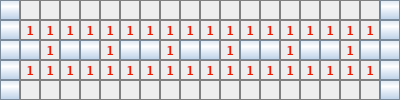
\includegraphics[width=0.45\hsize]{graphics/wire}}\\
\multicolumn{2}{c}{``Draht'' ohne Signal}\\
&\\
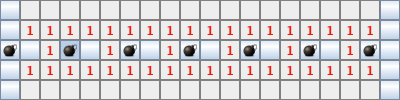
\includegraphics[width=0.45\hsize]{graphics/wire-0}&
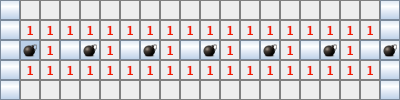
\includegraphics[width=0.45\hsize]{graphics/wire-1}\\
Bombenbelegung f"ur logisch ``0''&
Bombenbelegung f"ur logisch ``1''
\end{tabular}
\end{center}
\caption{Minesweeper-``Draht'', Spielplan mit zwei m"oglichen Bombenbelegungen,
die f"ur die zwei m"oglichen Zust"ande stehen k"onnen, die entlang des
Drahtes transportiert werden k"onnen.\label{minesweeper-wire}}
\end{figure}%

Dr"ahte m"ussen sich auch "uberkreuzen, in Abbildung~\ref{minesweeper-cross}
ist ein Spielplan mit zwei sich kreuzenden Dr"ahten gezeigt. Dieses
Kreuz kann zwei verschiedene Inputs vertikal und horizontal haben,
wie in Abbildung~\ref{minesweeper-crosses} dargestellt. Man kann
erkennen, dass sich die Zust"ande bei der Kreuzung gegenseitig nicht
ver"andern. Was links als Zustand 0 eingeht, wird auch rechts als Zustand
0 weitergeleitet.
\begin{figure}[H]
\begin{center}
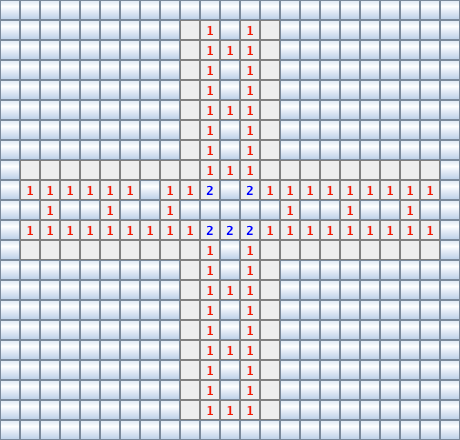
\includegraphics[width=0.6\hsize]{graphics/cross}
\end{center}
\caption{Kreuzung zweier ``Dr"ahte''\label{minesweeper-cross}}
\end{figure}%
\begin{figure}[H]
\begin{center}
\begin{tabular}{|l|c|c|}
\hline
\raisebox{12ex}{$0$}&
\raisebox{0pt}[0.4\hsize][0pt]{%
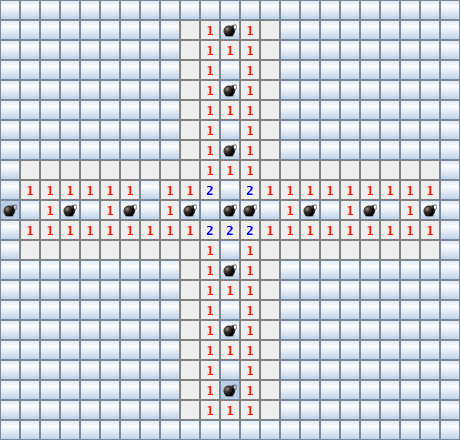
\includegraphics[width=0.41\hsize]{graphics/cross-11}}&
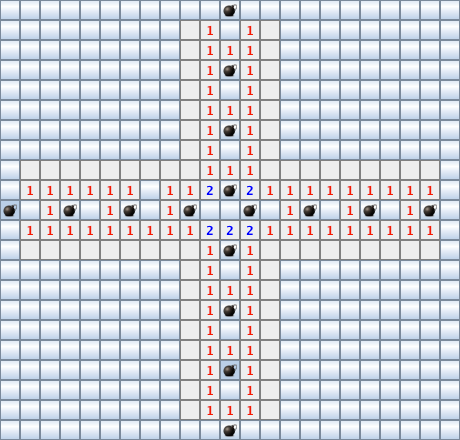
\includegraphics[width=0.41\hsize]{graphics/cross-10}\\
\hline
\raisebox{12ex}{$1$}&
\raisebox{0pt}[0.4\hsize][0pt]{%
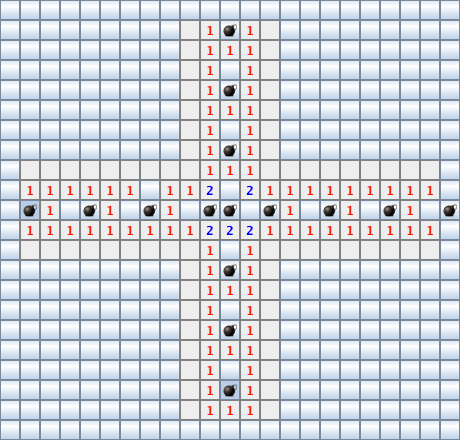
\includegraphics[width=0.41\hsize]{graphics/cross-01}}&
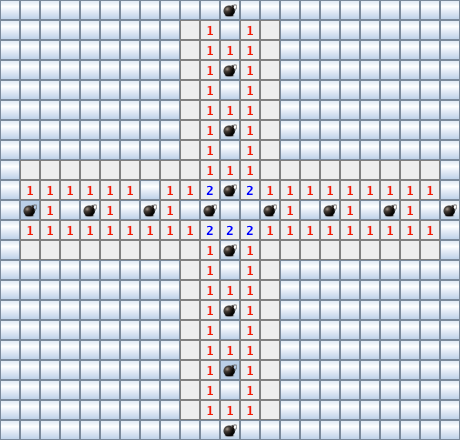
\includegraphics[width=0.41\hsize]{graphics/cross-00}\\
\hline
&\raisebox{0pt}[15pt][7pt]{$0$}&%
\raisebox{0pt}[15pt][7pt]{$1$}\\
\hline
\end{tabular}
\end{center}
\caption{Vier verschiedene m"ogliche Zustandskombinationen auf
einer Drahtkreuzung\label{minesweeper-crosses}}
\end{figure}%

Das NOT-Gatter muss aus einem Signal das invertierte Signal
machen. Dies schafft der Spielplan in Abbildung~\ref{splitter}.
Der von links eingespeiste Zustand wird rechts invertiert weitergeleitet.
Gleichzeitig wird der eingespeiste Zustand auch unver"andert nach
oben und unten abgeleitet, so dass man mit dieser Struktur auch
eine Aufteilung eines Signals in zwei Signale durchf"uhren kann.
\begin{figure}[H]
\begin{center}
\begin{tabular}{|c|c|c|c|}
\hline
\multirow{2}{0.4\hsize}{%
\raisebox{-5ex}[0.4\hsize][0pt]{%
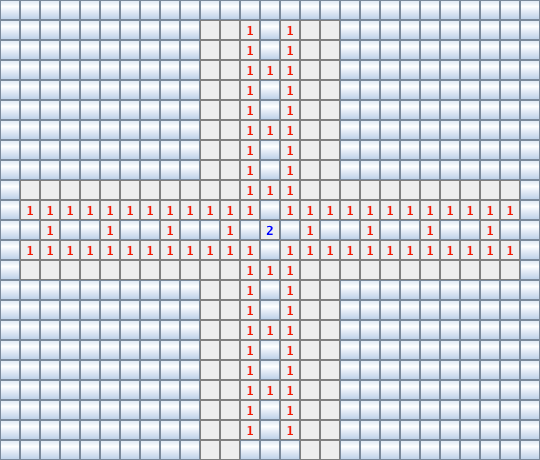
\includegraphics[width=\hsize]{graphics/splitter}%
}}&
\raisebox{11.5ex}{$0$}&
\raisebox{0pt}[0.35\hsize][0pt]{%
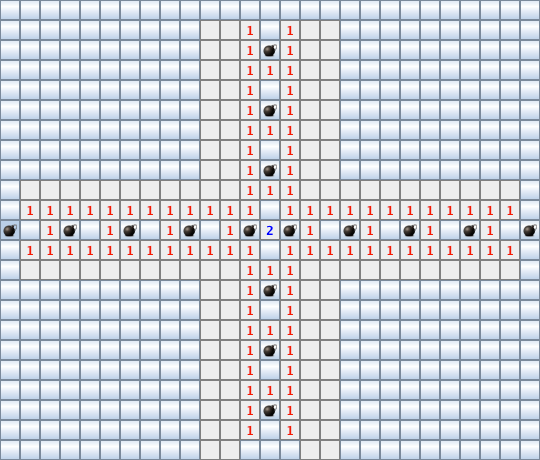
\includegraphics[width=0.4\hsize]{graphics/splitter-1}}&
\raisebox{11ex}{$1$}\\
\cline{2-4}
&
\raisebox{11.5ex}{$1$}&
\raisebox{0pt}[0.35\hsize][0pt]{%
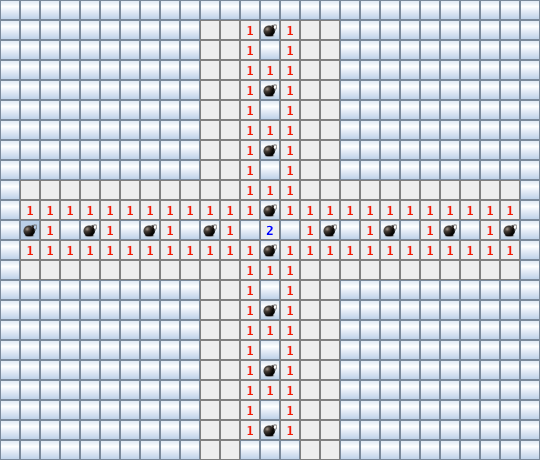
\includegraphics[width=0.4\hsize]{graphics/splitter-0}}&
\raisebox{11ex}{$0$}\\
\hline
\end{tabular}
\end{center}
\caption{NOT-Schaltung und Aufspaltung von Zust"anden\label{splitter}}
\end{figure}%

Damit bleibt nur noch das AND-Gatter. Dieses ist in Abbildung~\ref{andgate}
dargestellt, und in Abbildung~\ref{andstates} kann man die Funktion des
Gatters verfolgen.

\begin{figure}[H]
\begin{center}
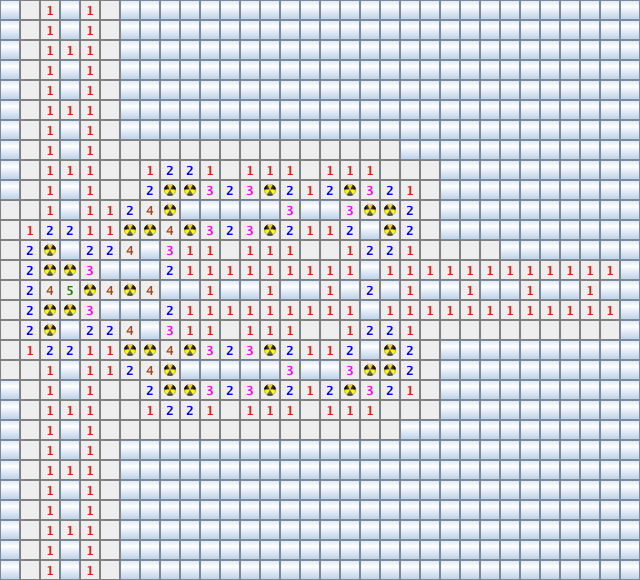
\includegraphics[width=0.55\hsize]{graphics/and}
\end{center}
\caption{Minesweeper-Spielplan f"ur das UND-Gatter\label{andgate}}
\end{figure}%
\begin{figure}[H]
\begin{center}
\begin{tabular}{|c|c|c|c|}
\hline
\raisebox{0pt}[13pt][4pt]{oberer Input}&unterer Input&Resultat&Output\\
\hline
\multirow{2}{10pt}{0}&%
\raisebox{11ex}{$0$}&%
\raisebox{0pt}[0.324\hsize][0pt]{%
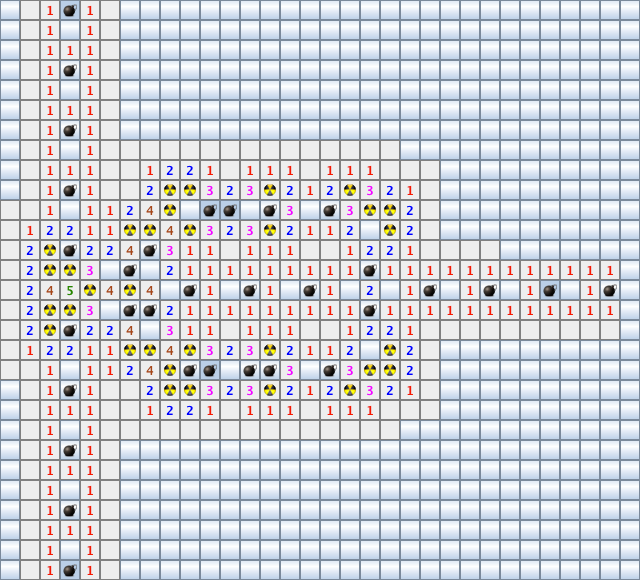
\includegraphics[width=0.342\hsize]{graphics/and-00}}&%
\raisebox{11ex}{$0$}%
\\
\cline{2-4}
&\raisebox{11ex}{$1$}&%
\raisebox{0pt}[0.324\hsize][0pt]{%
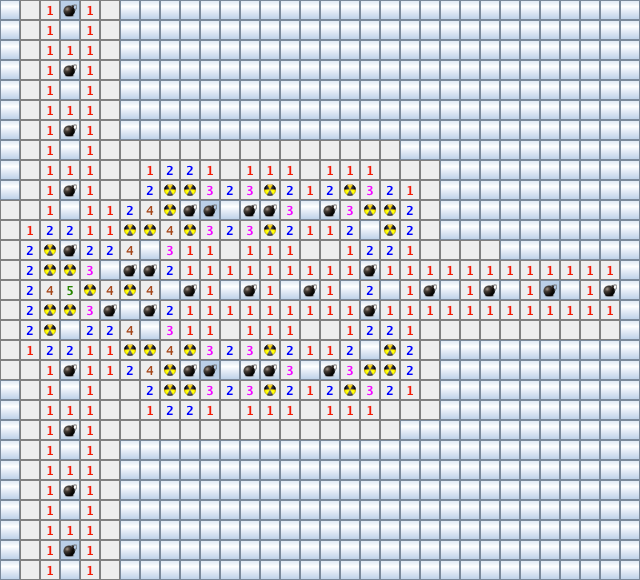
\includegraphics[width=0.342\hsize]{graphics/and-01}}&%
\raisebox{11ex}{$0$}%
\\
\hline
\multirow{2}{10pt}{1}&%
\raisebox{11ex}{$0$}&%
\raisebox{0pt}[0.324\hsize][0pt]{%
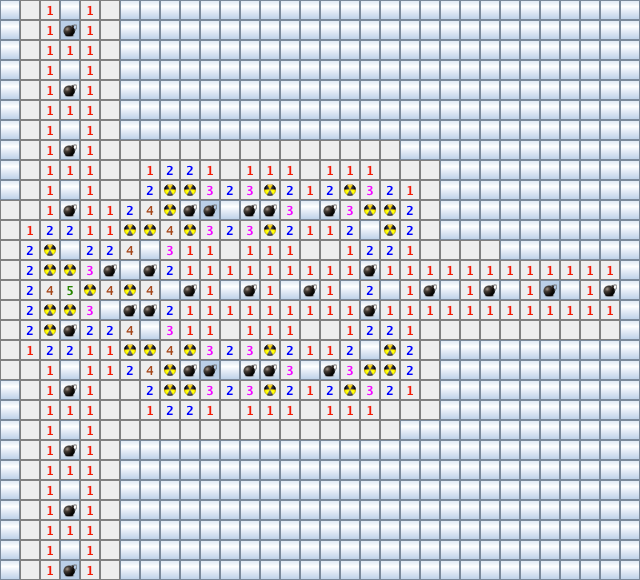
\includegraphics[width=0.342\hsize]{graphics/and-10}}&%
\raisebox{11ex}{$0$}%
\\
\cline{2-4}
&\raisebox{11ex}{$1$}&%
\raisebox{0pt}[0.324\hsize][0pt]{%
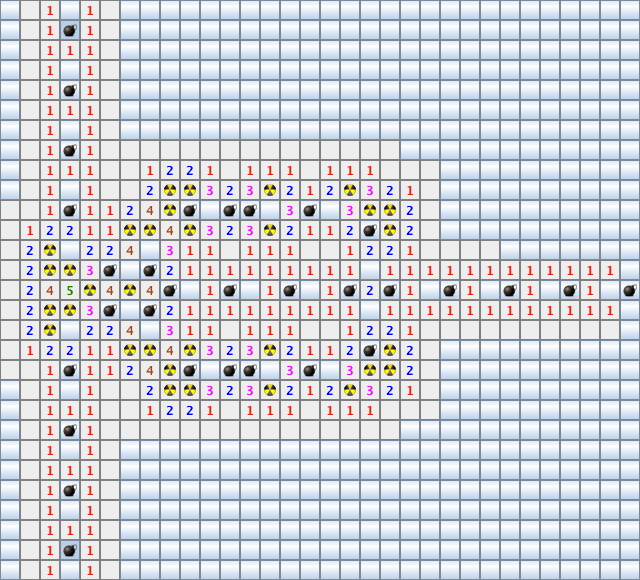
\includegraphics[width=0.342\hsize]{graphics/and-11}}&%
\raisebox{11ex}{$1$}%
\\
\hline
\end{tabular}
\end{center}
\caption{Nachweis der konsistenten ``Funktion'' des AND-Gatters
\label{andstates}}
\end{figure}%

Damit ist gezeigt, dass sich jede Schaltung in polynomieller Zeit in 
einen Minesweeper-Plan "ubersetzen l"asst. F"ur eine polynomielle
Reduktion wird aber verlangt, dass eine erf"ullbare Formel auf einen
Plan abgebildet wird, der am Ausgang eine logische 1 haben.
Da in unseren ``Dr"ahten'' eine logische 1 einer Bombe im zweiten
Feld (in Fortpflanzungsrichtung des Signals) entspricht, k"onnen
wir der Forderung nach einer logischen 1 dadurch Nachdruck verleihen,
dass wir diese letzte Bombe bereits platzieren. Als letzten Schritt
in der "Ubersetzung pflanzen wir also im ``letzten'' Feld eine Bombe.
Der so konstruierte Spielplan hat dann genau dann eine konsistente
Bombenbelegung, wenn der urspr"ungliche Schaltplan Output 1 haben kann.

Damit ist jetzt gezeigt, dass
\[
\text{\textsl{SAT}}\le_P
\text{\textsl{CIRCUIT}}\le_P\text{\textsl{MINESWEEPER-CONSISTENCY}},
\]
und weil \textsl{SAT} NP-vollst"andig ist, folgt auch, dass 
\textsl{MINESWEEPER-CONSISTENCY} NP-vollst"andig ist.

\subsection{Direkter Beweis}
Unter Verwendung der eben entwickelten Ideen k"onnte es m"oglich sein,
einen direkten Beweis der NP-Vollst"andigkeit von
\textsl{MINESWEEPER-CONSISTENCY} zu geben, ohne die Verwendung
von \textsl{SAT}. Dazu braucht man eine Theorie die besagt, dass
Schaltungen und Turing-Maschinen im wesentlichen "Aquivalent sind.
So eine Theorie existiert, und wird auch ben"otigt, um Turing-Maschinen
mit Quantencomputern vergleichen zu k"onnen. Letztere sind n"amlich
"uber ``Quantenschaltungen'' definiert. Dann sagt die Maschinerie des
vorangegangenen Abschnitts jedoch, dass man jede Turing-Maschine in
ein Minesweeper-Problem "ubersetzen kann, was NP-Vollst"andigkeit
beweist.
